\documentclass[
11pt, % The default document font size, options: 10pt, 11pt, 12pt
oneside, % Two side (alternating margins) for binding by default, uncomment to switch to one side
english, % ngerman for German
singlespacing, % Single line spacing, alternatives: onehalfspacing or doublespacing
%draft, % Uncomment to enable draft mode (no pictures, no links, overfull hboxes indicated)
%nolistspacing, % If the document is onehalfspacing or doublespacing, uncomment this to set spacing in lists to single
%liststotoc, % Uncomment to add the list of figures/tables/etc to the table of contents
%toctotoc, % Uncomment to add the main table of contents to the table of contents
%parskip, % Uncomment to add space between paragraphs
%nohyperref, % Uncomment to not load the hyperref package
headsepline, % Uncomment to get a line under the header
chapterinoneline, % Uncomment to place the chapter title next to the number on one line
%consistentlayout, % Uncomment to change the layout of the declaration, abstract and acknowledgements pages to match the default layout
]{MastersDoctoralThesis} % The class file specifying the document structure

\usepackage{textalpha}
\usepackage{amsmath}

\usepackage[backend=biber,style=numeric,sortcites,natbib=true,sorting=none]{biblatex}
\usepackage[utf8]{inputenc} % Required for inputting international characters
\usepackage[T1]{fontenc} % Output font encoding for international characters
\usepackage{todonotes}
\usepackage{mathpazo} % Use the Palatino font by default
\usepackage{adjustbox} % Resize table
%\usepackage[backend=bibtex,style=numeric-comp,sorting=none,natbib=true]{biblatex} % Use the bibtex backend with the authoryear citation style (which resembles APA)
\addbibresource{thesis.bib} % The filename of the bibliography
\usepackage{float}
\usepackage{graphicx}
\usepackage{rotating}
\usepackage[autostyle=true]{csquotes} % Required to generate language-dependent quotes in the bibliography
%\usepackage{glossaries}
\usepackage[T1]{fontenc}
\usepackage{comment}
\usepackage{hyperref}
%\makeglossaries
%\loadglsentries{glossary}


\newcommand{\vgp}{\textsc{vgpop }}
\newcommand{\bbp}{\emph{bubblepop }}
\newcommand{\bbc}{\emph{bubblecall }}
\author{Flavia Villani, Vincenza Colonna}
\date{1 June 2020}

\begin{document}
\begin{titlepage}
\centering
{\scshape\large\normalfont\bfseries UNIVERSITÀ DEGLI STUDI DI NAPOLI FEDERICO II \par}
 \vspace{0.7cm} 
{\scshape\large\normalfont Dipartimento di Medicina Molecolare e 

Biotecnologie Mediche
 \vspace{0.7cm} 
 
 
 
\includegraphics[width=0.25\textwidth]{fig/logo.png}
 \par
 \vspace{0.5cm}
\hspace{2cm}
 \par}
 \vspace{0.2cm}
{\scshape\large\normalfont CORSO DI LAUREA MAGISTRALE IN 

BIOTECNOLOGIE MEDICHE
 \par}
 \vspace{0.5cm} 
{\scshape\large\normalfont TESI DI LAUREA SPERIMENTALE IN GENETICA MEDICA
 \par}
  \vspace{0.5cm}
%{\scshape\large\normalfont\bfseries\textit Statistical analysis of selection using pangenomics data models
 %\par}
%{\scshape\large\normalfont\bfseries\textit \textit{vgpop}, a Python library for population genomics analyses from pangenomes
% \par}  

{\scshape\large\normalfont\bfseries\textit Population genomics analyses on{\scshape\large\normalfont\bfseries\textit 
 
 pangenome graphs
 \par}  


\vspace{1cm} 
\begin{minipage}{0.45\textwidth}
{\scshape\normalfont\large\bfseries Relatore:}\\
{\scshape\normalfont\large Dott. Vincenza Colonna} \\ 
{\scshape\normalfont\large\bfseries Relatore interno:} \\
{\scshape\normalfont\large Ch.mo Prof. Gabriella De Vita}\\
{\scshape\normalfont\large\bfseries Correlatore:} \\
{\scshape\normalfont\large Dott. Erik Garrison}
\end{minipage}
\hspace{2.5cm}
\begin{minipage}{0.25\textwidth}
{\scshape\normalfont\large\bfseries Candidato:}\\
 {\scshape\normalfont\large Flavia Villani \\
 matr. N79001438} 
\end{minipage}

\vfill
\centering
\vspace{0.48cm} 
{\scshape\Large\normalfont A.A. 2019/2020}

\end{titlepage}
%\maketitle
%----------------------------------------------------------------------------------------
%	LIST OF CONTENTS/FIGURES/TABLES PAGES
%----------------------------------------------------------------------------------------

\tableofcontents % Prints the main table of contents

%\listoffigures % Prints the list of figures

%\listoftables % Prints the list of tables


%--------------------------------------------------------------------------------------

% Chapter discussion

\chapter{Abstract} %-1pagina}
    
 % Main chapter title

\label{Chapter0} % For referencing the chapter elsewhere, use \ref{Chapter4} 

%----------------------------------------------------------------------------------------

% Define some commands to keep the formatting separated from the content 
\newcommand{\keyword}[1]{\textbf{#1}}
\newcommand{\tabhead}[1]{\textbf{#1}}
\newcommand{\code}[1]{\texttt{#1}}
\newcommand{\file}[1]{\texttt{\bfseries#1}}
\newcommand{\option}[1]{\texttt{\itshape#1}}

%~~~~~~~~~~~~~~~~~~~~~~~~~~~~~~~~~~~~~~~~~~~~~~~~~~~~~~~~~~~~~~~~~~~~~~~~~~~~~~~~~~~~~~~
Studies of genomes typically assume a single linear reference genome. This can make it difficult to observe sequences in other genomes that are divergent from the reference, which in turn can limit the accuracy and completeness of our analyses. To address this limitation, we can work with pangenome reference systems that represent the mutual relationships between many complete genomes without using a single one as a point of reference. These models often encode genomes and their mutual alignment in a compact graphical structure. Here, I begin the development of a software library for the statistical analysis of population genetic parameters of genomes stored in these graphical pangenomic data models. Because a pangenome embeds the linear genomes from which it is constructed, we can choose a particular reference genome and project the variants on it(which appear as bubbles in the graph). Therefore, I focused on develop algorithms for bubble detection, generating Variant Call Format (VCF) files directly from graphs. I then developed methods to annotate these variants with allele frequencies of genomes embedded in the input graph, and then explored the calculation of Fst. % for three different time points.

%\noindent
%We can use this variants projection to drive standard population genetic analyses. In my thesis, I focused on the calculation of Fst for three different time.



% Chapter discussion

\chapter{Introduction} %-5/10pagine} % Main chapter title

\label{Chapter2} % For referencing the chapter elsewhere, use \ref{Chapter4} 

%----------------------------------------------------------------------------------------

%1. Sequenziamento (mezza pagina)
%2. Modelli: genomica e pangenomica, facendo riferimento al problema reference based.
%3. come si codifica l'informazione: pangenoma (GFA) + bubble e vcf.
%4. HLA e polimorfico, complesso con modelli genomici 


%Grandezza genomi, genomi complessi, definizione pangenoma.


\section{DNA sequencing}
%TODO:
%1.Figura nanopore 
%2.referenze 
%3.  \url{https://ib.bioninja.com.au/standard-level/topic-3-genetics/32-chromosomes/genome-size.html}, aggiungere questo concetto, complessità degli organismi in giga, trovare articolo.


%PER ENZA \url{https://aulascienze.scuola.zanichelli.it/come-te-lo-spiego/2018/04/18/dal-metodo-sanger-a-oggi-40-anni-di-sequenziamento-del-dna/} mi sono ispirata a questi


The process of sequencing determines the exact order of the monomers in a biomolecule, the nucleotides in the case of DNA sequencing. Sequence analyses has many applications, such as identifing mutations or establish phylogenetic relationships among species. Sanger's method marked the beginning of genomics research and has been successfully until a decade ago when \textit{next generation sequencing (NGS)} was introduced to overcome the main limit of the Sanger sequencing,\cite{Sanger5463} i.e. the sequencing volume.

The main feature of NGS sequencing is the high-throughput. Unlike the traditional Sanger method, the NGS allows to analyze many sequences in parallel, reducing analysis times and costs. This reduction has improved over time: the sequencing of the first human genome, based on the Sanger method, required an investment of 2.7 billion dollars in about ten years \cite{ \footnote{Estimated in 1991 dollars, as per \url{https://www.genome.gov/human-genome-project/Completion-FAQ}}, while today the sequence of a human genome can be obtained for less than 1k dollars in one day \cite{sequencing}. Nevertheless, NGS has limitations too. One essential limitation is the initial amplification of DNA sequences, which can introduce random errors in the sequence and leads to the loss of "accessory" information, such as the constellation of epigenetic modifications that are important for understanding the function of a fragment of genome \cite{sequencing}. A second, and more severe limitation from the perspective of sequence analysis, is the short length of sequencing reads, which are typically shorter than 250bp. This greatly limits the fraction of a genome which can be accessed by this sequencing technology, and complicates the discovery and genotyping of structural variation.

To overcome these limitations, research is now pointing towards \textit{third generation} methods that are oriented toward sequencing very long regions (ideally whole chromosomes) without  prior amplification. Among these methods, nanopore sequencing derives from an observation from the 1980s that when a single-stranded DNA passes through a very narrow channel (nanopore) (Fig:\ref{fig:nanopore.png})generates a flow of ions with a characteristic pattern, which depends uniquely on its sequence. This technology allows sequencing millions of nucleotides without prior amplification of DNA fragments. \cite{wiki:nanopore}.

\begin{figure}[H]
\centering
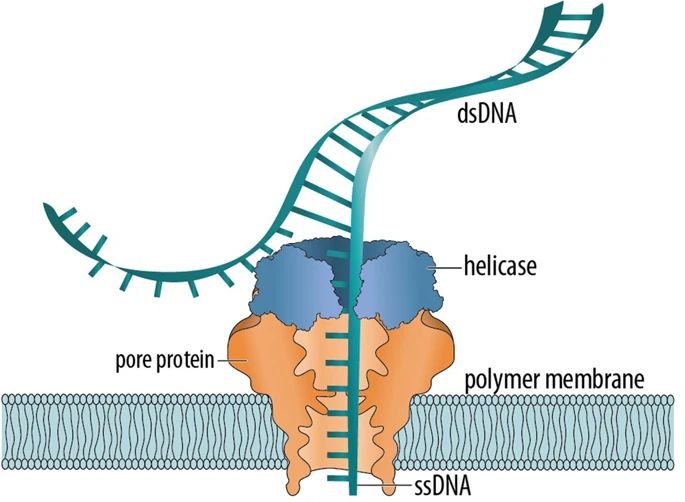
\includegraphics[width=0.70\textwidth]{fig/nanopore.png}
\decoRule
\caption{Schematic representation of a DNA molecule translocating a protein nanopore. The double-stranded DNA (dsDNA) is split by a helicase enzyme, allowing only a single strand (ssDNA) to pass while slowing it enough to achieve sufficient resolution for sequencing" \textit{Adapted from} \cite{sutton2019radiation}"} 
\label{fig:nanopore.png}
\end{figure}







\section{Genome \textit{versus} pangenome}
%TODO: REFERENCE BIAS chiedere ad Erik
%Genomics studies are based on two models: standard and alternative models. 

Standard approaches in sequence analysis relate sequences to a single linear reference genome. Sequence fragments produced by NGS are mapped and assembled against a reference genome, and genetic variants are identified through comparison with it. While being an efficient way of processing sequence information, this approach has a fundamental problem, i.e. substantial difference from the reference sequence are hard to observe and describe. This phenomenon is defined as \textit{reference bias}, i.e.  DNA fragments carrying the reference allele will be more likely to map successfully, or receive higher quality scores compared to alternate alleles. \cite{eizenga2020pangenome} 


Pangenomic methods allow to overcome limitations of the use of the reference genomes, relating all genomes directly to each other. In pangenomic approches, sequence and variation are combined. This practice is still new, and research into ways to design, implement, and apply this model is ongoing.  \cite{eizenga2020pangenome} 

In reference-based genomic analyses (\ref{fig:genomevspangenome.png} \textbf{a i}), all genomes (A–D) are compared with each other via their relationship to the reference genome (R).
In a pangenomic analyses (Figure \ref{fig:genomevspangenome.png} \textbf{a ii)},  all genomes are compared to each other, from which a particular reference is chosen arbitrarily. 
When extending the analysis with a new genome, (Figure \ref{fig:genomevspangenome.png} \textbf{a iii}) one adds it to the genomic model by comparing it with the reference genome.
In a pangenomic analyses instead (Figure \ref{fig:genomevspangenome.png} \textbf{a iv}), when a new genome is added, it is compared directly with all other genomes in the model.
 
 
% DA    qui in poi controllare con erik che si fa prima  
Regions of some genomes (\ref{fig:genomevspangenome.png} b) are unalignable against the reference and cannot be represented in a list of variants. A graphical model of the genomes allows a direct all-to-all comparison (\textbf{ii}), capturing all of their sequence relationships.

A collection of sequences representing a pangenome (\ref{fig:genomevspangenome.png} c). Multiple sequence alignment of the sequences captures their mutual relationships (\textbf{ii}).

(\ref{fig:genomevspangenome.png} d) In a de Bruijn graph, sequences are represented without bias, but variants may
correspond to larger graph structures. (\textbf{ii}) An acyclic sequence graph is equivalent to the multiple sequence alignment. (\textbf{iii}) A generic sequence graph can compactly represent a structural variant (shown in orange), using edges between the forward and reverse strands of
the graph to indicate the presence of an inversion.


\begin{figure}[H]
\centering
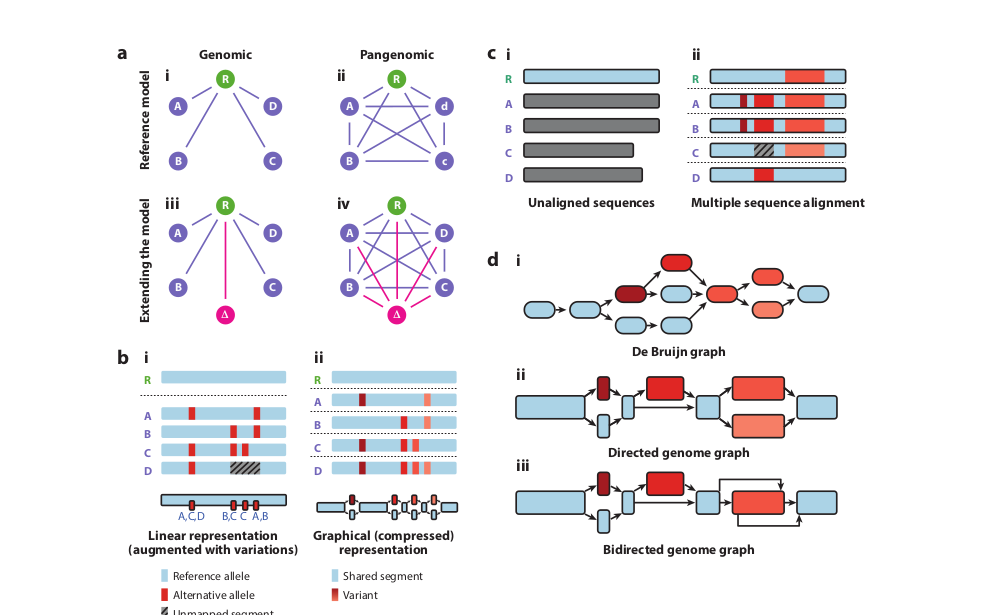
\includegraphics[width=1.00\textwidth]{fig/pangenome_genome.png}
\decoRule
\caption{Genomics versus pangenome (\textbf{A}), Linear representation with variants and Graphical representation compressed (\textbf{B})  Unaligned sequences and multiple sequence alignment (\textbf{C}), three types of graphs(\textbf{D}) \cite{eizenga2020pangenome}}
\label{fig:genomevspangenome.png}
\end{figure}


\section{Genetic variation in graphs}
%TODO: comment Type of variants by size and ability to detect them
The comparison of the sequence of multiple  genomes allow the identification of regions that present differences, i.e. genomic variants (Fig:\ref{fig:typeOfVariants}).  


\begin{figure}[H]
\centering
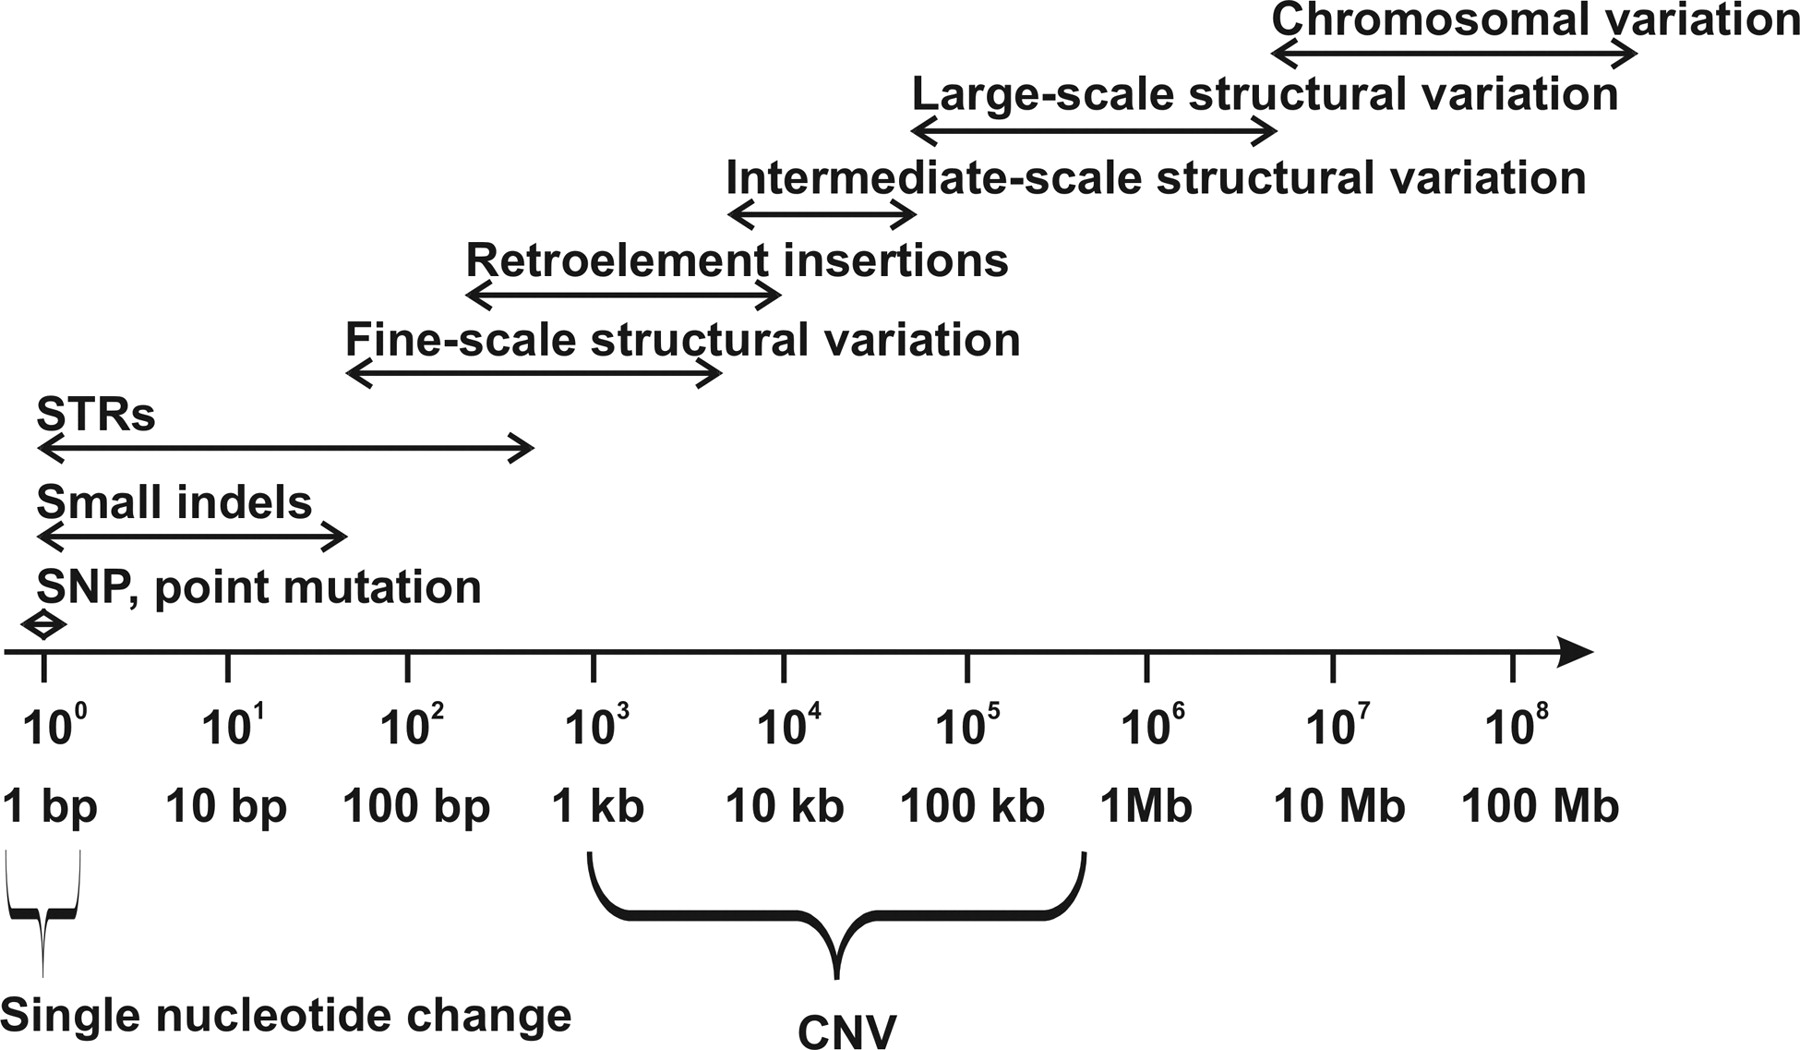
\includegraphics[width=0.7\textwidth]{fig/typeOfVariants.jpeg}
\decoRule
\caption{\textbf{Type and size of genetic variants.}"\textit{Adapted from} \cite{pollex2007copy}"} 
\label{fig:typeOfVariants}
\end{figure}

In graphs genetic variants appear as circles or \textit{bubbles}. In the handlegraph there are five important elements described in Figure \ref{fig:gfa.png}:
\begin{itemize}
\item\textbf{Nodes} represented by yellow rectangles. Each node is associated with a numeric ID and a sequence. 

\item\textbf{Strand Forward and reverse}. DNA strands have forward (+) and reverse (-) orientation. Each node contains a forward and reverse handle (red solid and dashed rectangles, respectively). Handles show the node identifier, the direction (+ or -), and the sequence of the handle.

\item\textbf{Edges} are connections between nodes, repesented by arrows in the figure.

\item\textbf{Paths} are obtained by 'walking' through the graph and represent the actual sequences. Not necessarily all possible paths should be observed in a set of real data.

\item\textbf{Steps} describe paths visits to nodes strands.
\end{itemize}

In (Figure \ref{fig:gfa.png}) the first two paths differ by a single nucleotide polymorphism, with one passing through 2+:T, and the other through 3+:G. The third path is the reverse complement of the first. The fourth is the same as the first, but contains an inversion, passing through 5-: AATC rather than 5+: GATT.



\begin{figure}[H]
\centering
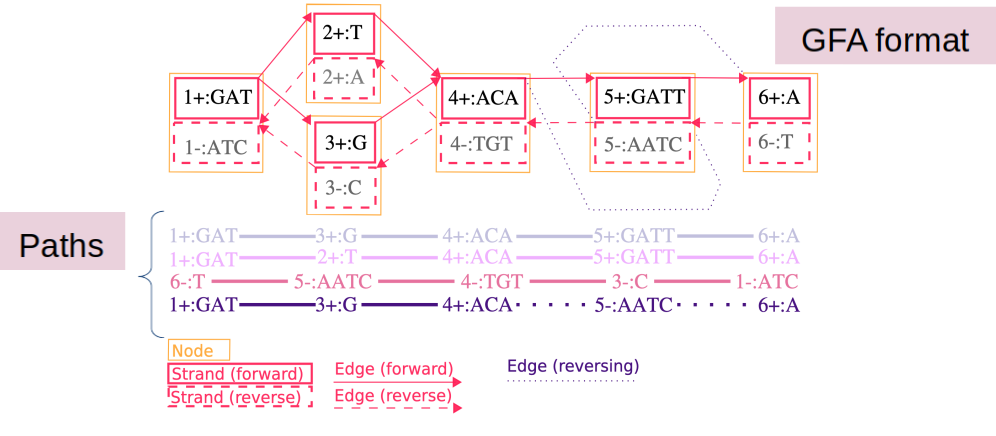
\includegraphics[width=1.00\textwidth]{fig/GFA.png}
\decoRule
\caption{Entities in the bidirected sequence graph (\textbf{A}) \cite{eizenga2020succinct}}
\label{fig:gfa.png}
\end{figure}

When only two variants (of one or more bases) are present, the bubble looks like a circle, while less simple patterns are referred as \textit{superbubbles} (Figure \ref{fig:sup_bub.png})
%Variants are coding in the graph as bubbles. 

\begin{figure}[H]
\centering
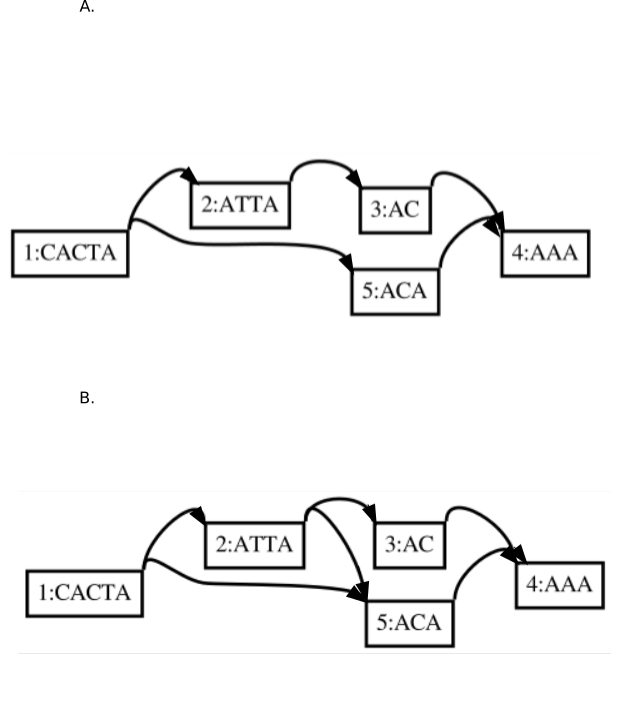
\includegraphics[width=0.50\textwidth]{fig/bub_sup.png}
\decoRule
\caption{Bubble(\textbf{A}), Superbubble (\textbf{B})}
\label{fig:sup_bub.png}
\end{figure}


The superbubble is a more complex subgraph type in which a set of (not necessarily disjoint) paths start and end at common source and sink nodes.\cite{paten2018superbubbles}.
Refering the definition from \cite{onodera2013detecting}, any pair of distinct vertices equation in a digraph (Fig: \ref{fig:sup_bub.png}A):
%OK x e y e X se le metti anche sulla figura altrimenti e' diffcile seguire 
\begin{enumerate}
\item reachability: y is reachable from x.

\item matching: The set of vertices, X, reachable from x without passing through y is equal to the set of vertices from which y is reachable without passing through x (passing through here means to enter and then exit a vertex on the path).

\item acyclicity: The subgraph induced by X is acyclic.

\item minimality: No vertex in X other than y forms a pair with x that satisfies the criteria previously defined, and similarly for y.


\end{enumerate}

%I'm concentred for \textit{bubblepop} to a case specific of a superbubble i.e  bubbles (Fig: \ref{fig:sup_bub.png})
In my project I focused on a specific case of a superbubble i.e. a bubble (Fig: \ref{fig:sup_bub.png}) to implement the core function of the library that is named \textit{bubblepop}. 

A bubble consists of multiple directed unipaths from a vertex\textbf{ v} to a vertex \textbf{u} and is commonly caused by a small number of errors in the centre of reads.\cite{brankovic2016linear}. The bubble may be generalized to the idea of a superbubble, which is a directed, acyclic component of a graph with a single head and tail node.\cite{onodera2013detecting}.

A homologous sequence corresponding to the common start
and end nodes in the bubble flanks two or more alternative alleles in the middle.\cite{garrison2019graphical}.Bubbles can nest and contain more complicated internal structures between the paths
through them. 

\section{Coding of genetic information}

When the genomic information is coded with linear model it is stored in files in Variant Call Format(VCF), whereas graphical representation of a pangenome are stored in Graphical Fragment Assembly (GFA). 



\subsection{Variant Call Format}
Variant Call Format (VCF) is a text file format and is a generic format for storing DNA polymorphism data such as SNPs, insertions, deletions and structural variants, together with rich annotations. (\cite{10.1093/bioinformatics/btr330}). 


\begin{figure}[H]
\centering
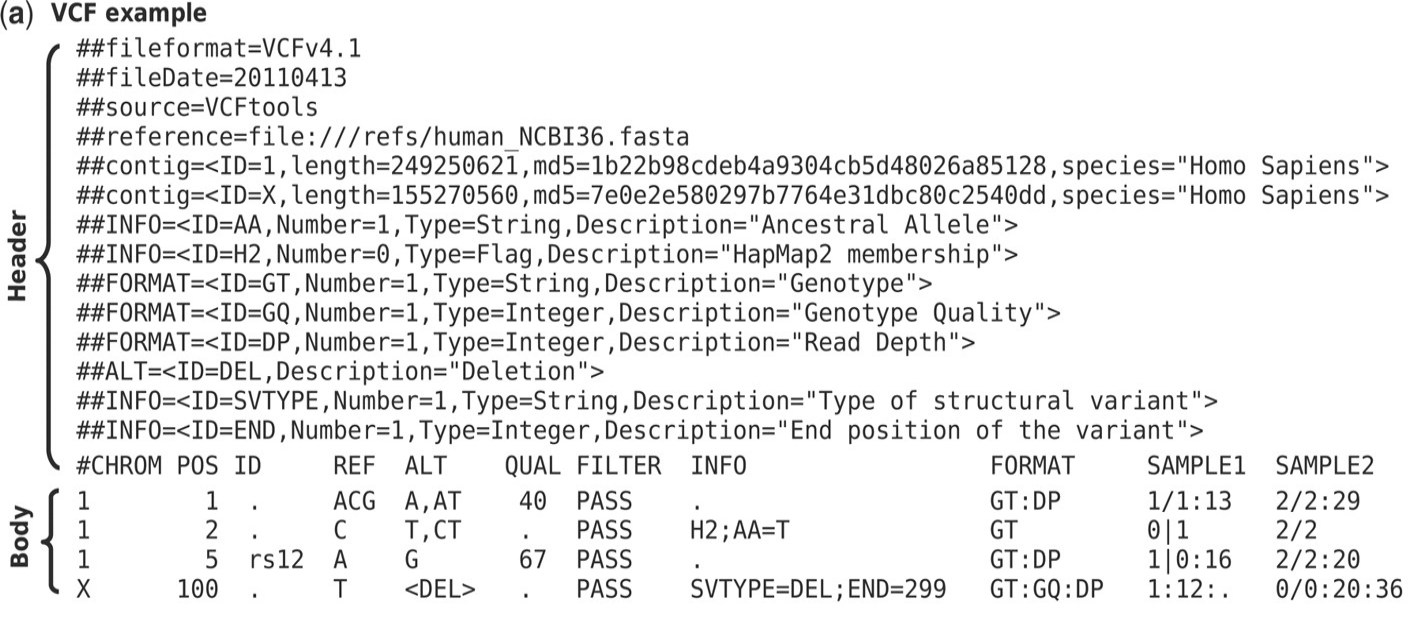
\includegraphics[width=1.00\textwidth]{fig/vcf.png}
\decoRule
\caption{AMPLIARE (\textbf{A}), Linear representation with variants (VCF)) Fig:\cite{10.1093/bioinformatics/btr330}}
\label{fig:vcf.png}
\end{figure}



VCF file (\ref{fig:vcf.png}) consists of:
\begin{itemize}

\item\textbf{Header section}

In the (Fig: \ref{fig:vcf.png}) adapted by (\cite{10.1093/bioinformatics/btr330}) the header contains an arbitrary number of information lines, each starting with characters \#\#, and a TAB delimited field definition line, starting with a single \#,
character. The meta-information header lines provide a standardized description of tags and annotations used in the data section. The use of meta-information allows the information stored within a VCF file to be tailored to the data set in question. It can be also used to provide information about the means of file creation, date of creation, version of the reference sequence, software used and any other information relevant to the history of the file. 

\item\textbf{Data columns}

These corresponding to data columns representing the chromosome (CHROM), a 1-based position of the start of the variant (POS), unique identifiers of the variant (ID), the reference allele (REF), a comma separated list of alternate non-reference alleles (ALT), a phred-scaled quality score (QUAL), site filtering information (FILTER) and a semicolon separated list of additional, user extensible annotation (INFO). In addition, if samples are present in the file, the mandatory header columns are followed by a FORMAT column and an arbitrary number of sample IDs that define the samples included in the VCF file. The FORMAT column is used to define the information contained within each subsequent genotype column, which consists of a colon separated list of fields.

\end{itemize}


\subsection{Graphical Fragment Assembly}

Pangenome data are represented by Graphical Fragment Assembly (GFA, \cite{GFA})

\begin{figure}[H]
\centering
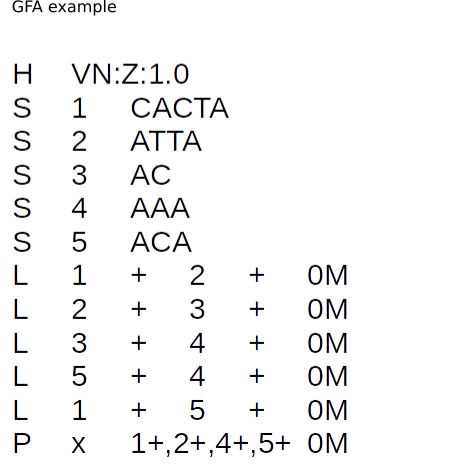
\includegraphics[width=0.50\textwidth]{fig/GFAexample.png}
\decoRule
\caption{Graph representation)} 
\label{fig:GFAexample.png}
\end{figure}

%GFA fatto da me, non copiato, usato per disegnare la bubble della figura precedente 


GFA format is a representation of variation in genomes, splice graphs in genes.





\begin{itemize}

\item\textbf{Header section} start with H.
\item\textbf{Segment line} start with S.
Segment a continuous sequence or subsequence.
\item\textbf{Link lines} start with L.
Link an overlap between two segments. Each link is from the end of one segment to the beginning of another segment. Containment an overlap between two segments where one is contained in the other.
\item\textbf{Path lines} start with P. 
Path an ordered list of oriented segments, where each consecutive pair of oriented segments are supported by a link record.

%dire che ci sono linee opzionali


\end{itemize}

\section{HLA}

\begin{figure}[H]
\centering
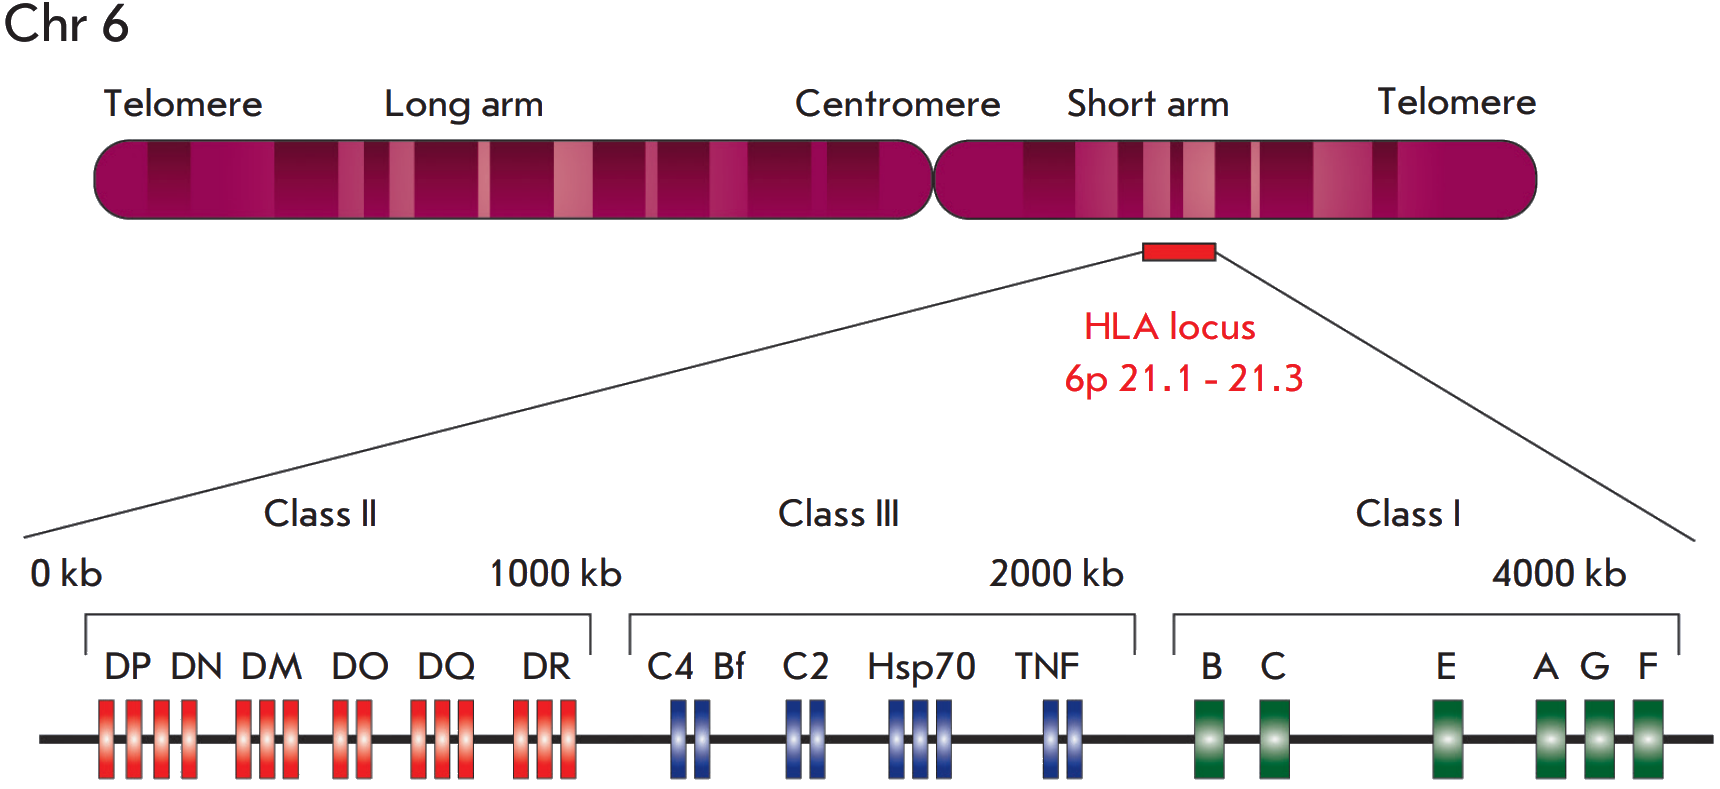
\includegraphics[width=0.80\textwidth]{fig/HLA_loci.png}
\decoRule
\caption{Schematic representation of the HLA locus on human chromosome 6. adapted from \cite{zakharova2019contribution})}
\label{fig:HLA.png}
\end{figure}




The human major histocompatibility complex (MHC) or human leukocyte antigen (HLA) is a locus composed of closely linked polymorphic genes that code for cell surface proteins essential for the adaptive immune system. It contains several gene clusters coding surface heterodimeric proteins, which are anchored to the plasma membrane and are responsible for antigen presentation to T cells, a stage that is followed by the development of an adaptive immune response. MHC proteins are subdivided into class I, class II, and class III (the complement system) \cite{campbell1993map}. Many genetic diseases are caused by mutations in this region \cite{tiwari2012hla}.  


The HLA region (Fig.\ref{fig:HLA.png}) is located on the short arm of chromosome 6 from 6p21.1 to p21.3 in a region spanning 7Mb. The class II region includes genes for the $\alpha$ and $\beta$ chains of the MHC class II molecules HLA-DR, HLA-DP and HLA-DQ. In addition, the genes encoding the DM$\alpha$ and DM $\beta$ chains, as well as the genes encoding the $\alpha$ and $\beta$ chains of the DO molecule (DO $\alpha$ and DO $\beta$, respectively), are also located in the MHC class II region.





In the latest version of the human reference genome (GRCh38), there are several alternate loci where the sequence variation is too complex to be represented with a single sequence \cite{eggertsson2017graphtyper}. These loci are generally highly polymorphic, and many are known to co-segregate with disease and are therefore of great interest in population genetics. The most prominent example, the HLA region, is known to associate with a number of human diseases . 

Short-read sequencing is the standard in genome-wide sequence analysis. Most common approaches for discovering sequence variants involve aligning sequence reads to a reference genome \cite{li2009fast} and searching for variants as alternative sequences in read alignments. However, some reads cannot be aligned to a reference genome, particularly those originating from highly polymorphic regions and regions absent from the reference genome.

% Chapter discussion

\chapter{Results of the Research Group-5/10pagine} % Main chapter title

\label{Chapter3} % For referencing the chapter elsewhere, use \ref{Chapter4} 

%----------------------------------------------------------------------------------------

Descrive il progetto di ricerca di cui fa parte l’attività sperimentale svolta dal candidato. Vanno qui riportati i risultati ottenuti dal gruppo di ricerca in precedenza e/o in contemporanea rispetto all’attività svolta dal candidato che siano rilevanti per l’argomento della tesi. Nel caso in cui il candidato abbia svolto, nell’ambito del gruppo di appartenenza, un progetto di ricerca nuovo e autonomo, questa sezione può essere eliminata. In questa sezione è richiesto l’uso di illustrazioni.

% Chapter discussion

\chapter{Aim of the thesis} %-1,2 pagine} % Main chapter title

\label{Chapter4} % For referencing the chapter elsewhere, use \ref{Chapter4} 

%----------------------------------------------------------------------------------------

%Illustra in modo chiaro e coinciso le finalità del lavoro sperimentale svolto dal candidato. 


Standard studies in sequence analysis typically assume a single linear reference genome (VCF). 
These models have some limits, as structural and complex variation can render these simplified models inapplicable. With this model another limit is that see the information that there are presents in the reference sequence. To address this limitation, the aim of my thesis is work to implement a software library for the statistical population analysis using pangenomic data models.\\ 

These are Typically represented in the Graphical Fragment Assembly (GFA) format, these models can represent whole genome alignments in a compact graphical structure. Because they embed the linear genomes from which they are constructed, I can choose a particular reference genome and project the variants (which appear as bubbles in the graph) back into any reference frame. I have focused for the first step on algorithms for bubble detection that allow us to generate Variant Call Format (VCF) files from graphs.\\

I use this projection to drive standard population genetic analyses, and as a mechanism to communicate results that we obtain from pangenome graph based population genetic analyses which I am designing.
In the second step, I use functions of library for analyses directly on pangenome data.




%%% PRomemoria, 20 pagine
APPUNTI:
-quando si allinea con il riferimento si vede 'solo' quello che c'è nel riferimento

\vspace{2cm}
Introduzione:
- allineamento usando la sequenza di riferimento, limiti nell'usare la sequenza di riferimento, approccio pangenomica.

Nella conversione di gfainvcf il core è l'identificazione delle bubble

Genoma di sars-cov2, focalizzarsi su TIME CONSUMING   


%Tabella  (scrivere meglio descrizioni )
%bubblePop & Bubble detection
%gfa2vcf &  rewrite file in gfa format in a vcf 
%gfa2allelefreq & explanation 
%gfa2genofreq & explanation 
%gfa2fst & explanation 
%devo spiegare nel dettaglio le funzioni in termine di codice o di cosa fanno? 
%Aggiungere anche mstovcf,seqgentogfa?

1. descrizione vgpop (6 pagine entro 5 giugno ) 
1a. Bubble detection
1b. variant calling 
1c. validation 
1d. allelic and genotipic frequencies, Fst 

2. application to simulated data (6 pagine entro 6 giugno) 
2a. simulation scenario and tools 
2b. application of vgpop to simulated data 

3. Study cases: (6 pagine) 


- covid19
allele frequencies from pangenome 
De-novo assembly
- yeast 
allele frequencies

% Chapter results

\chapter{Results achieved by the Candidate} % Main chapter title

\label{Chapter5} % For referencing the chapter elsewhere, use \ref{Chapter4} 

%----------------------------------------------------------------------------------------



%~~~~~~~~~~~~~~~~~~~~~~~~~~~~~~~~~~~~~~~~~~~~~~~~~~~~~~~~~~~~~~~~~~~~~~~~~~~~~~~~~~~~~~~


%%%%%%%%%%%%%%%%%%%%%%%%%%%%%%%%%%%%%%%%%%%%%%%%%%%%%%%%%%%%%%%%%%%%%%%%%%%%%%%%%%%%%%%
%  Section 
%%%%%%%%%%%%%%%%%%%%%%%%%%%%%%%%%%%%%%%%%%%%%%%%%%%%%%%%%%%%%%%%%%%%%%%%%%%%%%%%%%%%%%%

%\section{Description vgpop}
\section{Implementation of the \vgp library}  

I developed a library named \vgp to conduct standard population genetics analyses using pangenomic data models. Typically represented in the Graphical Fragment Assembly (GFA) format, these models can represent whole genome alignments in a compact graphical structure. The library is written in Python programming language under MIT license; the code is publicly available on GitHub (\url{https://github.com/Flavia95/VGpop}) 

At its present state \vgp contains five functions briefly introduced in tab \ref{tab:functionvgpop} and detailed in the following paragraphs.

\vspace{1cm}

{\small
\begin{table}[H]
\caption{Functions implemented in \vgp}
\label{tab:functionvgpop}
\centering
\begin{adjustbox}{width=0.80\textwidth}
\begin{tabular}{c c c c }
\toprule
\tabhead{vgpopfunction} & \tabhead{Description} & Input & Output \\
\midrule
bubblepop & Identification of polymorphic genomic regions (bubbles) &  GFA & dictionary  \\
gfa2vcf & Conversion of files in GFA format to VCF format & GFA & VCF \\
gfa2allelefreq & Calculation of allele frequencies & GFA & allelefreqfile \\
gfa2genofreq & Calculation of genotype frequencies & GFA & genotypefrequenciesfile \\
gfa2fst & Calculation of F\textsubscript{ST} & GFA & fstfile\\
\bottomrule\\
\end{tabular}
\end{adjustbox}
\end{table}
}

%\vspace{1cm}

%%%%%%%%%%%%%%%%%%%%%%%%%%%%%%%%%%%%%%%%%%%%%%%%%%%%%%%%%%%%%%%%%%%%%%%%%%%%%%%%%%%%%%%%%%%%
%  Subsection 
%%%%%%%%%%%%%%%%%%%%%%%%%%%%%%%%%%%%%%%%%%%%%%%%%%%%%%%%%%%%%%%%%%%%%%%%%%%%%%%%%%%%%%%%%%%%


\subsection{Bubblepop}

The main challenge of my project was to extract the information about variable sites (i.e. regions where more that one type of sequence is present) from the graphs. Any population genetic analysis is in fact based on the information contained in the variable segments of the sequence and their occurrence in the population under investigation. Because of their appearance in the pangenome graph, variable sites are referred to as bubbles (Figure \ref{fig:gfa.png}). \\

The core of \vgp is the \bbp function, which takes as input a pangenome, detects bubbles, and outputs the sequences of the variants contained in the bubbles.

\bbp takes as input a GFA file and gives as output a dictionary, i.e. a table of correspondences between region of the graph and sequence variants. It explores the graph using the two recursive algorithms described in the following paragraphs and works in two consecutive steps. 

%% non servono le lettere, zzom dalontano, graph piu' complesso senza dettaglio si fa vdere DFS sceglie un nodo  eesplora a casa un pezzoee  
%tree con root piu' lontana, aggiungere un pezzo di root 

\begin{figure}[H]
\centering
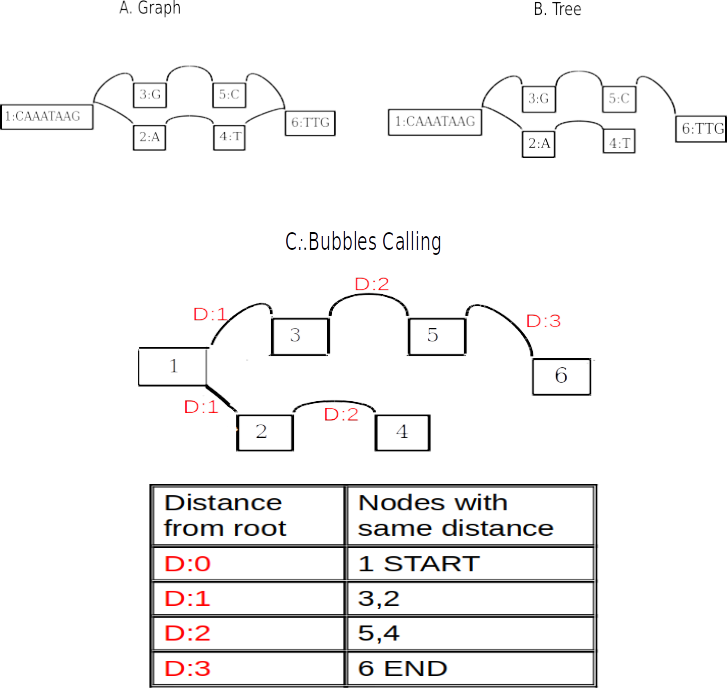
\includegraphics[width=1.00\textwidth]{fig/bubblepop.png}
\decoRule
\caption{\textit{bubblepop} transforms a pangenome (\textbf{A}) in a tree (\textbf{B}) using two algorithms, the Depth First Search and the Breadth first Search. On tree identify bubble (\textbf{C})}
\label{fig:bubblepop.png}
\end{figure}


\setcounter{secnumdepth}{3}
\subsubsection{Step 1: Depth first Search}

%I use two recursive algorith \cite{geeksforgeeks.org}.%questo e' un sito generico
The Depth First Search (DFS) \cite{korf1985depth,wiki:DFS} is a recursive algorithm for searching graph data structures. DFS select an arbitrary node as root node and explores as far as possible along each branch. The exploration process runs until some depth cutoff is reached, and then DFS backtracks to the next most recently expanded node. Therefore, only the path of nodes from the initial  node to the current  node  must be stored in order to execute the algorithm (Figure \ref{fig:bubblepop.png}A))

%vertex==node? non capisco questo paragrafo
DFS marks each vertex of a graph as visited. With this, start by one of the vertices of the graph in a stack. Take the item on top of the stack and add it to the list visited. Create a list of the adjacent nodes of that vertex. Add node that is not in the visited list.\\

In \bbp I use the DFS algorithm to explore the graph starting from a random node of the pangenome. At each iteration, \bbp creates a spanning tree from the part of the pangenome that is explored (Figure \ref{fig:bubblepop.png}B), threfore transforming the pangenome in a set of trees.\\ %vediamo meglio questo: Starting from the pangenome graph, with the DFS algorithm a spanning tree of its vertices is obtained.\\

A tree is an entity that describes relationships between objects (Figure \ref{fig:phylogenies.jpg}). The tips of the tree are called leaves; leaves are connected by branches, whose length is proportional to the observed differences between the leaves; the coalescence of two branches generates a node or vertex. In phylogeny and evolutionary genetics the nodes indicate the most common ancestor of sequences. In trees obtained from pangenomes, the branches are obtained by resolving the bubble in its edges components and the nodes represent chunks of sequences, the root of the tree is a special node located at the beginning of the tree. 

%aggiungere due colori uno per pangenomica uno per evolutonary, la figura serve per ora e per dopo
\begin{figure}[H]
\centering
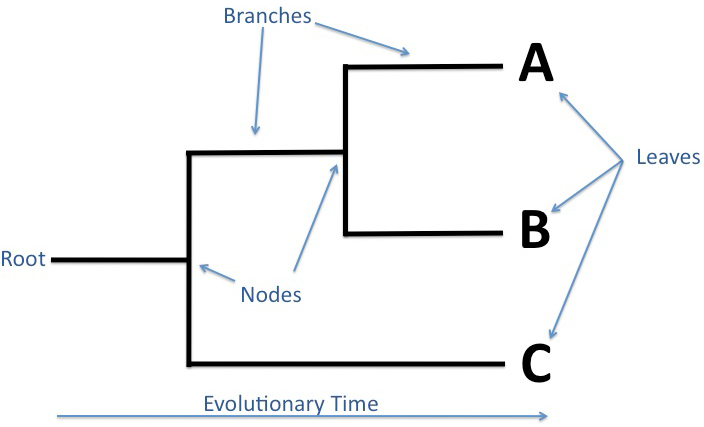
\includegraphics[width=0.80\textwidth]{fig/phylogenies.jpg}
\decoRule
\caption{\textbf{Fig: phylogenetic tree}. 
\url{modified from https://arthropoda.wordpress.com/2010/01/19/introduction-to-phylogenetics/}}
\label{fig:phylogenies.jpg}
\end{figure}

\subsubsection{Step 2: Breadth first Search}
Breadth First Search (BFS) \cite{beamer2012direction} is another recursive algorithm for traversing or searching tree or graph data structures. I used BFS on the trees obtained applying DFS (Figure \ref{fig:bubblepop.png}B).

When used on trees, at each iteration BFS starts at the tree root and explores all of the neighbor nodes at one step, then expands to the nodes at the next steps until a goal state is reached \cite{korf1985depth, wiki:BFS}. The information encountered during the exploration is recored. 
%come per BFS quest aparte no nmi e' chiara, no capisco cosa vuoi dire, da migliorare 
With this start by putting any one of the three's vertices at the back of a queue.Take the front item of the queue and add it to the visited list. Create a list of that vertex's adjacent nodes. Add the ones which aren't in the visited list to the back of the queue. \url{https://www.programiz.com/dsa/graph-dfs}

In \bbp, I used BFS to the trees obtained by DFS (Figure \ref{fig:bubblepop.png}B).
%distance of a.... leave?
In particular with BFS I calculated the distance of a node from the root node of the tree and stored this information in a dictionary, i.e. a table of correspondence (Figure \ref{fig:bubblepop.png}). 


\subsubsection{\bbc}
Once the pangenome has been decomposed with \bbp in a set of trees whose information are stored in dictionary, \bbp make explicit the content of the bubbles and its position along a chosen reference sequence.    

Within the dictionary, the beginning and the end nodes of a bubbles are identified by the fact that their distance from the root is uniqe, i.e. they are the only nodes with a specific distance from the tree. (Figure \ref{fig:bubblepop.png}C). All other nodes are  inner nodes of bubbles and correspond to variable regions of the sequence, furthermore nodes with the same distance from the root are in the same bubble.\\

\bbc works in X steps

\begin{itemize}


\item\textbf{Possible paths and reference }
Considering all the possible paths %COME SI FA? v aspiegato % 
As implemented now, the first path in the GFA file is used as reference, however it is possible to set any available paths as reference.

\item{variant calling }  A variant is a nodes supported by at least one path, whose sequence is different from the sequence of the corresponding node in the chosen reference.

\item\textbf{SNV and INDEL}
For Deletion if the considerate node in the REF is the current node in the current path, it means that in the current path a node is missing, so there is a deletion respect to the REF.
For Insertion if the considerate node in the current path is the current node in the ref, it means that in the current path there is a node that is missing in the REF, that is an insertion.

For SNV if the sequence are different in the current path respect to the REF.

\item \textbf{variant positioning} The variants are called respect to a path chosen as reference%NON E' vero, la posizione e' rispetto al REF .
\end{itemize}

%I obtained VCF.






%%%%%%%%%%%%%%%%%%%%%%%%%%%%%%%%%%%%%%%%%%%%%%%%%%%%%%%%%%%%%%%%%%%%%%%%%%%%%%%%%%%%%%%%%%%%
%  Subsection 
%%%%%%%%%%%%%%%%%%%%%%%%%%%%%%%%%%%%%%%%%%%%%%%%%%%%%%%%%%%%%%%%%%%%%%%%%%%%%%%%%%%%%%%%%%%%

\setcounter{secnumdepth}{3}
\subsection{gfa2vcf}
%tolto the second, non c'e un ordine 
The \textit{gfa2vcf} function of \vgp takes as input a graph in the GFA format and output a corresponding linear representation in the VCF format. To do this \textit{gfa2vcf} uses first \bbp to decompose the pangenome in a set of trees and then \bbc to transform the information of the graph in a linear format. 


%PER LA FIGURA: va completata con una parte che fa vedere il GFA e se vuoi il VCF risulatante da questa bolla forse si puo' mettere questo esempio semplice e uno piu' complesso 
\begin{figure}[H]
\centering
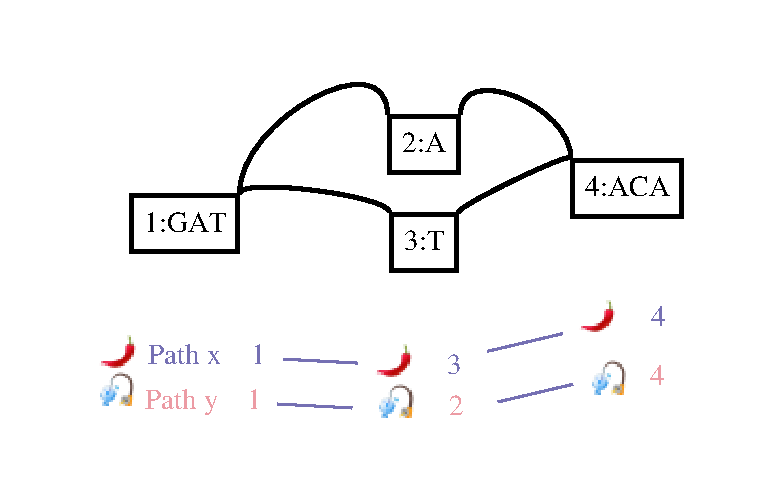
\includegraphics[width=1.10\textwidth]{fig/GraphchrXnew.pdf}
\decoRule
\caption{\textbf{Fig A: Bubble}. Path x represents the sequence used as a reference to describe variants that are present in a sequence analysed.} %aggiungere path
\label{fig:bubble.png}
\end{figure}


%FIGURA FORSE NON necessaria 
%\begin{figure}[H]
%\centering
%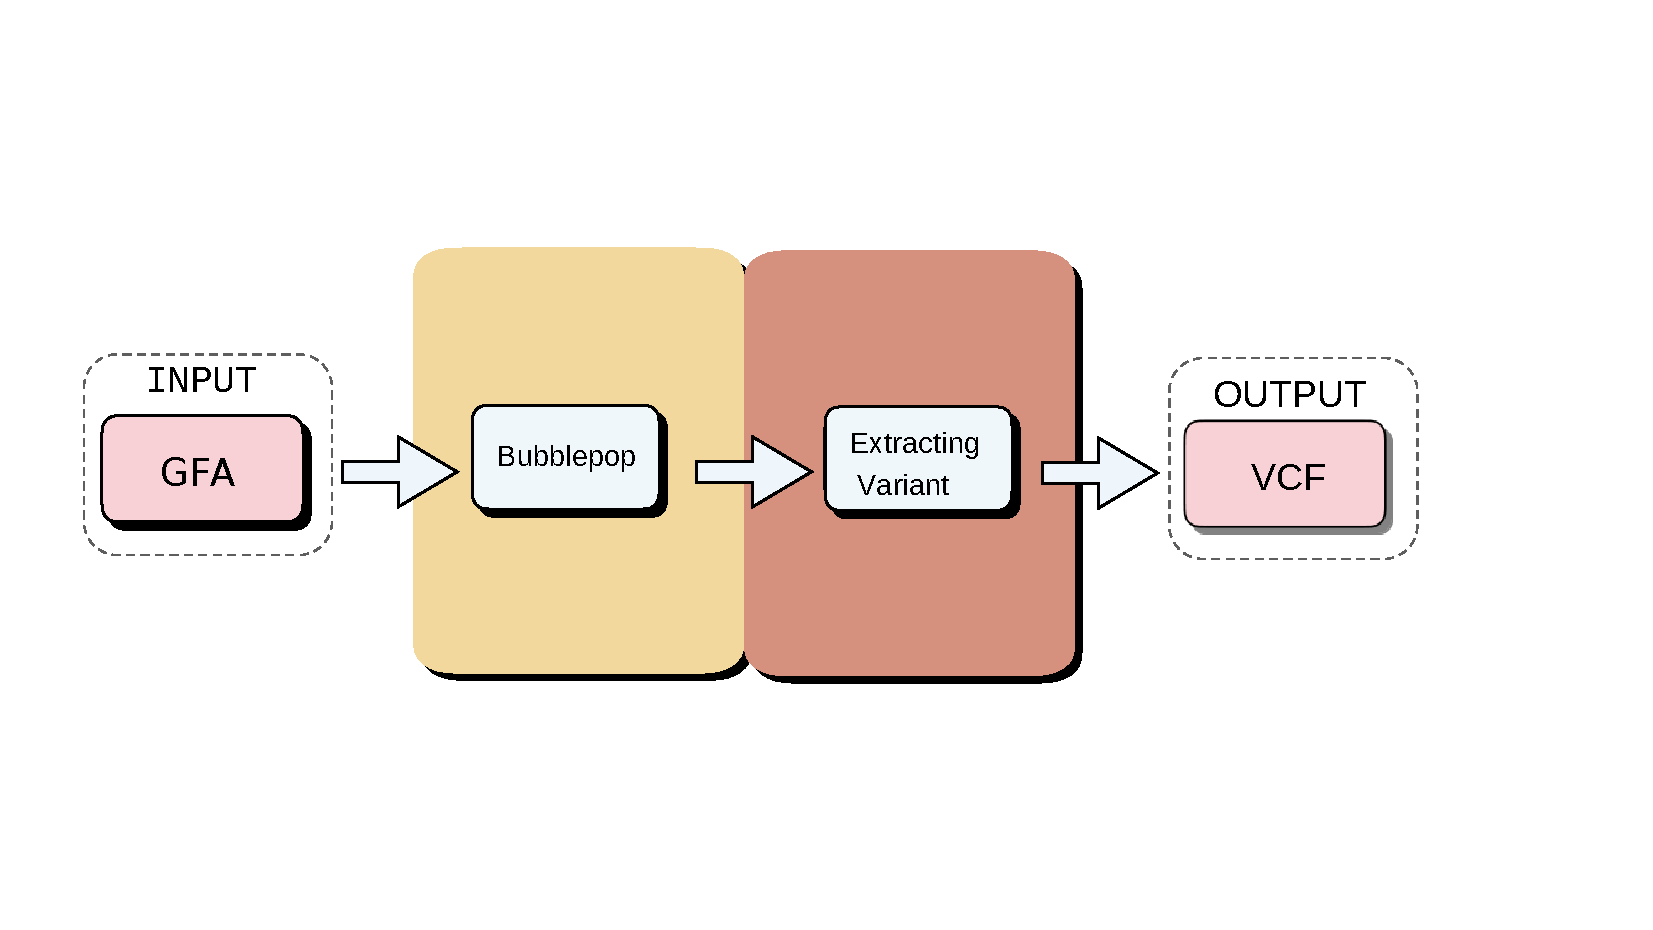
\includegraphics[width=1.10\textwidth]{fig/gfatovcfnew.pdf}
%\decoRule
%\caption{\textbf{Graph} GfatoVcf}
%\label{fig:vgpop.pdf}
%\end{figure}


% non erano  chiare le definizioni di GFA, rest ail dubbio su SNV indel 
{\small
\begin{table}
\caption{Correspondences between elements of the GFA and VCF}
\label{tab:gfatovcf}
\centering
\begin{adjustbox}{width=0.50\textwidth}
\begin{tabular}{c c}
\toprule
\tabhead{GFA} & \tabhead{VCF} \\
\midrule
 Path Name & CHROM \\
 Position in the reference sequence & POS \\
 Sequence of bubble's inner nodes & REF allele  \\
  that is present in the path chosen as reference  &  \\
 Sequence of bubble's inner nodes & ALT allele  \\
  that is NOT present in the path chosen as reference  &  \\
 SNV, INDEL & Type\\
\bottomrule\\
\end{tabular}
\end{adjustbox}
\end{table}
}

%non farei una sub sub section 
%\subsubsection{Validation of the VCF obtained with \textit{gfa2vcf}}
To validate the VCF obtaind using \textit{gfa2vcf}, I reconstructed a graph starting from it and using an existing tool, i.e. the functions \textit{vgconstruct} and \textit{vgview} from the \textsc{vgtool} library (Figure \ref{fig:validationgraph.png}A, adapted from \cite{vg}, (QUESTA VA COME REFERENZA \url{https://nicedoc.io/vgteam/vg}). Visual comparison of the graph used as input of \textit{gfa2vcf} and the one reconstructed with \textsc{vgtool}, shows a complete correspondence of the two graphs, suggesting that the \textit{gfa2vcf} works well (Figure \ref{fig:validationgraph.png}B).  

%PERCHE' ripeter la definizione id variaton graphs?
%Variation graphs provide a succinct encoding of the sequences of many genomes. 
%A variation graph (in particular as implemented in vg) is composed of:
%\begin{itemize}
%\item nodes: which are labeled by sequences and ids
%\item edges: which connect two nodes via either of their respective ends
%\item paths: describe genomes, sequence alignments, and annotations (such as gene models and transcripts) as walks through nodes connected by edges
%\end{itemize}
%Tools in vg maintain paths as immutable during transformations of the graph. They use paths to project graph-relative data into reference-relative coordinate spaces. Paths provide stable coordinates for graphs built in different ways from the same input sequences.

%%cambiare GFA start con GFA from \vgp  e GFA con GFA from \textsc{vgtools} DIDALSCALIA GIA@ CAMBIATA  
\begin{figure}[H]
\centering
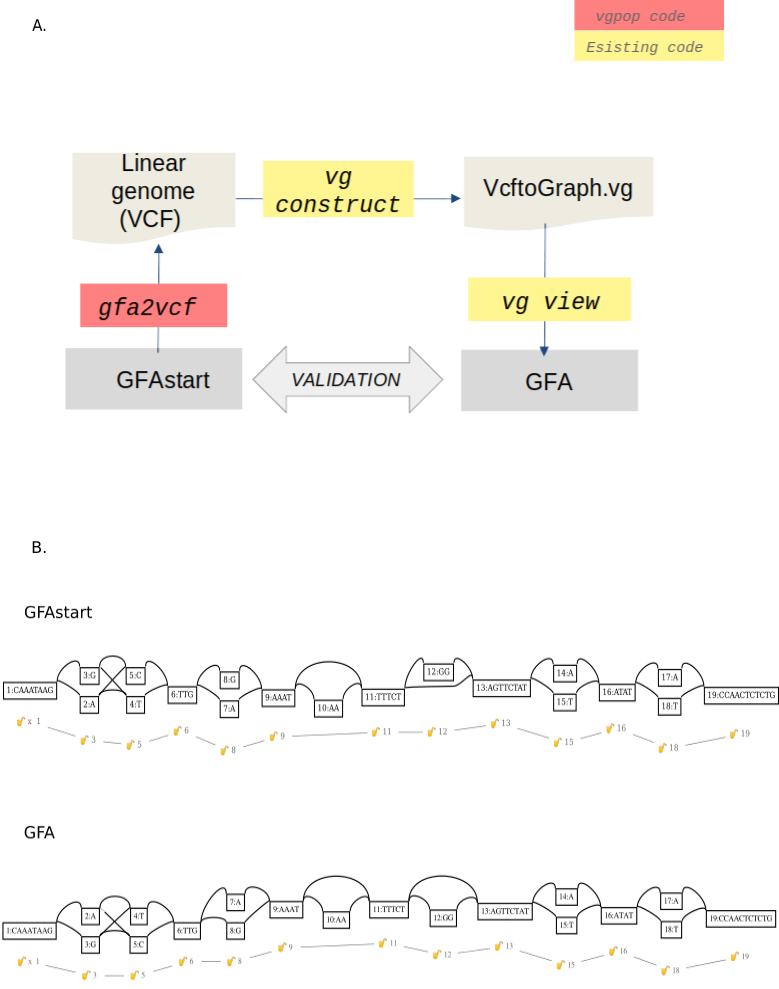
\includegraphics[width=1.00 \textwidth]{fig/validationgfa2.vcf.png}
\decoRule
\caption{Validation scheme of the \textit{gfa2vcf} function (\textbf{A}). the graph used as input from \vgp is identical to the one reconstructed using \textsc{vgtools} from the VCF obtained by \textit{gfa2vcf} (\textbf{B})}
\label{fig:validationgraph.png}
\end{figure}

%%%%%%%%%%%%%%%%%%%%%%%%%%%%%%%%%%%%%%%%%%%%%%%%%%%%%%%%%%%%%%%%%%%%%%%%%%%%%%%%%%%%%%%%%%%%
%  Subsection 
%%%%%%%%%%%%%%%%%%%%%%%%%%%%%%%%%%%%%%%%%%%%%%%%%%%%%%%%%%%%%%%%%%%%%%%%%%%%%%%%%%%%%%%%%%%%

\subsection{gfa2allelefreq} 

The \textbf{frequency of an allele} is an indication of how common the allele is in a population. It is calculated by counting how many times the allele appears in the population, dividing by the total number of copies of the gene.\\

For a locus with \emph{p} alleles, the allele frequency of the \emph{i\textsubscript{th}} allele \emph{p\textsubscript{i}} in a population of haploid individuals is: \\

Haploid allele frequency    $p\textsubscript{i} = \dfrac{i}{N}$\\

\noindent
where \emph{i} is the count of the alleles and \emph{N} is the number of individuals in the population.\\
\noindent
In a diploid populations the formula becomes: \\

Diploid allele frequency  $p\textsubscript{i} =  \dfrac{i}{2N}$$\\

%The \textbf{frequency of a genotype} is the count of the genotype occurrence in the population. A locus with two alleles, \textit{A} and \textit{B} has three possible genotypes: \textit{AA, AB, BB}.  
%frequency of B $q = {f(BB)} + \dfrac{1}{2} f(AB)$

The \textit{gfa2allelefreq} function of \vgp takes as input a GFA format and output a file that contains the calculation of allele frequencies for variable loci. In \textit{gfa2allelefreq} the allele frequency correspond to the 



%In this specific case I obtained two file of calculation, one from each population. 

This calculation start with \textit{bubblepop}, after detection of bubble I calculate allele frequencies, for each variants the number of  paths  are  calculate  that  support  the  variant node divided  by  total  number  of  paths(considered even REF).
Only allele frequencies different from 1 were considered. 
 

%%%%%%%%%%%%%%%%%%%%%%%%%%%%%%%%%%%%%%%%%%%%%%%%%%%%%%%%%%%%%%%%%%%%%%%%%%%%%%%%%%%%%%%%%%%%
%  Subsection 
%%%%%%%%%%%%%%%%%%%%%%%%%%%%%%%%%%%%%%%%%%%%%%%%%%%%%%%%%%%%%%%%%%%%%%%%%%%%%%%%%%%%%%%%%%%%


\subsection{gfa2genfreq}

The fourth function of \vgp is the \textit{gfa2genfreq}, which takes as input a GFA format, and as output a file that contains the calculation of genotype frequencies.

Genotype frequencies \cite{brooker2014principles} in a population is the number of individuals with a given genotype divided by the total number of individuals in the population. In population genetics, the genotype frequency is the frequency or proportion of genotypes in a population. 

$f(a) = \dfrac{(Aa) + 2 x (aa))}{2 x (AA) + 2 x (Aa) + 2 x (aa)}$

I counted ATGC in a position and I checked the reference base and calculate for each allele the frequency (count/numhaplotype).


%%%%%%%%%%%%%%%%%%%%%%%%%%%%%%%%%%%%%%%%%%%%%%%%%%%%%%%%%%%%%%%%%%%%%%%%%%%%%%%%%%%%%%%%%%%%
%  Subsection 
%%%%%%%%%%%%%%%%%%%%%%%%%%%%%%%%%%%%%%%%%%%%%%%%%%%%%%%%%%%%%%%%%%%%%%%%%%%%%%%%%%%%%%%%%%%%


\subsection{gfa2fst}

The fifth function of \vgp is the \textit{gfa2$F\textsubscript{st}$}, which takes as input allele frequencies file, and as output a file that contains the calculation of $F\textsubscript{st}$.

The fixation index is a measure of population differentiation due to genetic structure. It is frequently estimated from genetic polymorphism data, such as single-nucleotide polymorphisms (SNP) or microsatellites developed as a special case of
the Wright’s fixation index ($F\textsubscript{st})$ is a measure of population differentiation due to genetic structure. 

It can be estimated as the standardized variance of allele frequencies among sub-populations.

$F\textsubscript{st} = \dfrac{s^{2}}{p(1-p)}$

with s and p being the variance and mean, respectively, of the allele frequency. 

$F\textsubscript{st}$ \cite{barbujani2010human} ranges from 0, when all sub-populations are identical, to 1, when different alleles are fixed in different sub-populations.


The central points of this function are three:



\begin{itemize}
\item\textbf{Mean of  allele frequencies}:  obtained by \textit{gfa2allelefreq} from two populations. These frequencies represent 
\begin{verbatim}
mean = statistics.mean([freq_pop1, freq_pop2])
\end{verbatim}
 
\item\textbf{Calculation of $F\textsubscript{st}$}

\begin{verbatim}
fst = statistics.pvariance([freq_pop1, freq_pop2])/((mean)*(1-mean))
\end{verbatim}
\item\textbf {Mean of $F\textsubscript{st}$} from 100 replicate. 

\begin{verbatim}
mean_fst_list.append(statistics.mean(fst_list))
\end{verbatim}
\end{itemize}




\vspace{8cm}


%%%%%%%%%%%%%%%%%%%%%%%%%%%%%%%%%%%%%%%%%%%%%%%%%%%%%%%%%%%%%%%%%%%%%%%%%%%%%%%%%%%%%%%
%  Section 
%%%%%%%%%%%%%%%%%%%%%%%%%%%%%%%%%%%%%%%%%%%%%%%%%%%%%%%%%%%%%%%%%%%%%%%%%%%%%%%%%%%%%%%

\section{Application to simulated data}
I exploited analyses of genetic population on simulated data to already know what to expect.


%%%%%%%%%%%%%%%%%%%%%%%%%%%%%%%%%%%%%%%%%%%%%%%%%%%%%%%%%%%%%%%%%%%%%%%%%%%%%%%%%%%%%%%%%%%%
%  Subsection 
%%%%%%%%%%%%%%%%%%%%%%%%%%%%%%%%%%%%%%%%%%%%%%%%%%%%%%%%%%%%%%%%%%%%%%%%%%%%%%%%%%%%%%%%%%%%

\subsection{Simulation Scenario and Tools}

\subsubsection{MS}

I used MS \cite{hudson2004ms}, a program to generate samples under a variety of neutral models. The purpose of this program is to allow one to investigate the statistical properties of such samples, to evaluate estimators or statistical tests, and generally to aid in the interpretation of polymorphism data sets.

The program ms can be used to generate many independent replicate samples under a variety of assumptions about migration, recombination rate and population size. I simulated two populations that are divided into three different times. I expected Fst to be greater for the two populations more distantly divided over time.(T3)

%forse citare nei metodi pacchetto usato per fare i plot?




\begin{figure}[H]
\centering
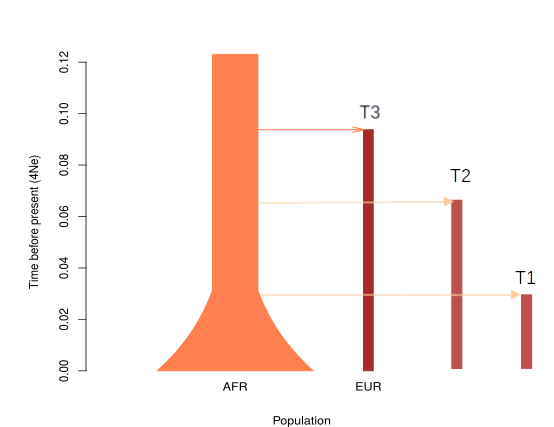
\includegraphics[width=1.10\textwidth]{fig/populationthreetime.png}
\decoRule
\caption{\textbf{Fig:Population}. 
T1 (0.031254 Ne), T2(0.0625 Ne),T3(0.09375 Ne)}
\label{fig:population.pdf}
\end{figure}

\begin{verbatim}
In the first case I simulated two populations that divided 5.000 generations ago.


ms 80 100 -t 11.2 -I 2 40 40 -g 1 44.36 -n 2 0.05 -eg 0.03125 1 0.0 -ej 0.03125 2 1   

I simulated two populations that divided 10.000 generations ago.

ms 80 100 -t 11.2 -I 2 40 40 -g 1 44.36 -n 2 0.05 -eg 0.03125 1 0.0 -ej 0.0625 2 1   

I simulated two populations that divided 15.000 generations ago.

ms 80 100 -t 11.2 -I 2 40 40 -g 1 44.36 -n 2 0.05 -eg 0.03125 1 0.0 -ej 0.09375 2 1   
\end{verbatim}

Explanation the parameters of ms:

\begin{itemize}
\item\textbf{nsam<nsample>:}
is the number of copies of the locus in each sample.

\item\textbf{nrep<nreplicate>:}
is the number of independent samples to generate;


\item\textbf{t <mutationrate>:}
is equal to $$4N0\mu$$ where N0 is the diploid population size and where u is the neutral mutation rate for the entire locus;

\item\textbf{I <individual>:}
followed by the number of subpopulations,npop, and the sample configuration. The sample configuration is a list of npop integers (n 1 n 2...) indicating the number of chromosomes sampled from each subpopulation;

\item\textbf{g <growth>:}
 it indicate the growth of pop1 at a definite time;

\item\textbf{n:}
it set growth of population 2 at time; 

\item\textbf{eg <growth rate>:}
pop1 stop growing at time 0.03125;

\item\textbf{ej <join>:}
Pop1 join with pop2. It is the parameter that change in three command. 

I convert mstogfa but I need the information about the links between the bubbles.  

\subsubsection{Seq-Gen}
I needed the whole sequence rebuilt and the links between the bubbles """SPIEGARE PERCHE' E/O PER FARCI COSA.

Seq-Gen \cite{rambaut1997seq} is a program that will simulate the evolution of nucleotide sequences along a phylogeny, using common models of the substitution process. A range of models of molecular evolution are implemented, including the general reversible model. 

Seq-Gen requires a tree as input, therefore I added the parameter -T to all the MS commands to obtained a tree as output. With seq-gen, I reconstructed the sequences for the three different simulated times.

\begin{verbatim}
seq-gen -mHKY -l 40 -s .2 -wa -z 783763255346462154 <treems40popT1> T1.seqgen

seq-gen -mHKY -l 40 -s .2 -wa -z 783763255346462154 <treems40popT2> T2.seqgen

seq-gen -mHKY -l 40 -s .2 -wa -z 783763255346462154 <treems40popT3> T3.seqgen

\end{verbatim}

Explanation of parameters:

\begin{itemize}

\item\textbf{m <MODEL>:} This option sets the model of nucleotide or amino acid substitution.
\item\textbf{l <SEQUENCELENGTH>:} This option allows the user to set the length in nucleotides or amino acids that each simulated sequence should be.
\item\textbf{s <SCALE>:} This option allows the user to set a value with which to scale the branch lengths in order to make them equal the expected number of substitutions per site for each branch. Basically Seq-Gen multiplies each branch length by this value.
\item\textbf{z <RANDOMNUMBERSEED>:} This option allows the user to specify a seed for the random number generator. Using the same seed (with the same input) will result in identical simulated datasets. This is useful because you can then delete the (often large) simulated sequence files to save disk space. To recreate a set of simulations, you must use exactly the same model options. The default is to obtain a seed from the system clock which will be displayed on the screen allowing it noted down.
\item\textbf{wa:}
Write Ancestral Sequences. This option allows the user to obtain the sequences for each of the internal nodes in the tree obtained with ms 
\end{itemize}

\end{itemize}

\subsection{Application vgpop}
\begin{figure}[H]
\centering
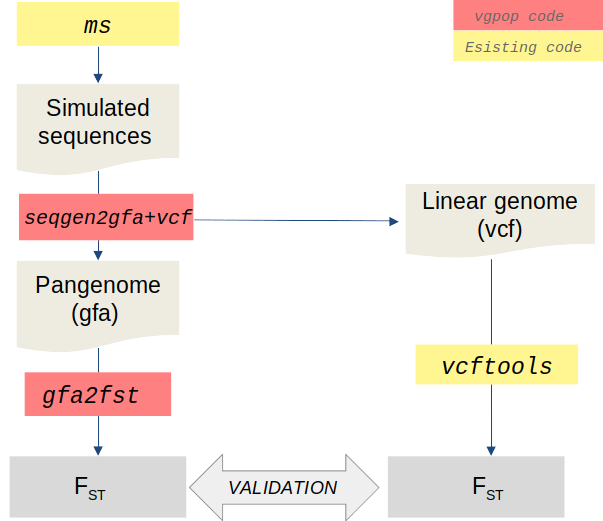
\includegraphics[width=1.00\textwidth]{fig/pipeline_new.png}
\decoRule
\caption{\textbf{Fig:Pipeline}. 
Validation.}
\label{fig:pipeline.pdf}
\end{figure}

Starting from ms, I obtained simulated sequences, I reconstruct an ancestral tree with Seq-Gen. 

These sequences were encoded in a GFA file and VCF file with \textit{seqgen2gfa+vcf }.


On GFA file I calculate the allele frequencies with \textit{gfa2allelefreq}, the genotype frequencies with \textit{gfa2genofreq}, and the Fst with \textit{gfa2fst}. 

On VCF file I extract individuals from the populations that I considered with bcftools. %non so se mettere questa parte
\begin{verbatim}

bcftools view -S pop_1.txt seqgen.vcf.gz -o seqgen.bcf.vcf.gz #pop1
bcftools view -S pop_2.txt seqgen.vcf.gz -o  seqgen.bcf.vcf  #pop2 
\end{verbatim}

Calculate Allele Frequencies for two populations with vcftools
\begin{verbatim}

vcftools --vcf seqgen.bcf.vcf --freq --out seqgen.bcf.pop1.vcf .frq

vcftools --vcf ms_rep{1}.bcf.vcf --freq --out seqgen.bcf.pop2.vcf.frq 

\end{verbatim}

I calculate Fst with \textit{vcf2fst} (aggiungerlo nell'immagine?). %aggiungere altre info sullo script

Fst is the same from GFA and VCF file.


\begin{figure}[H]
\centering
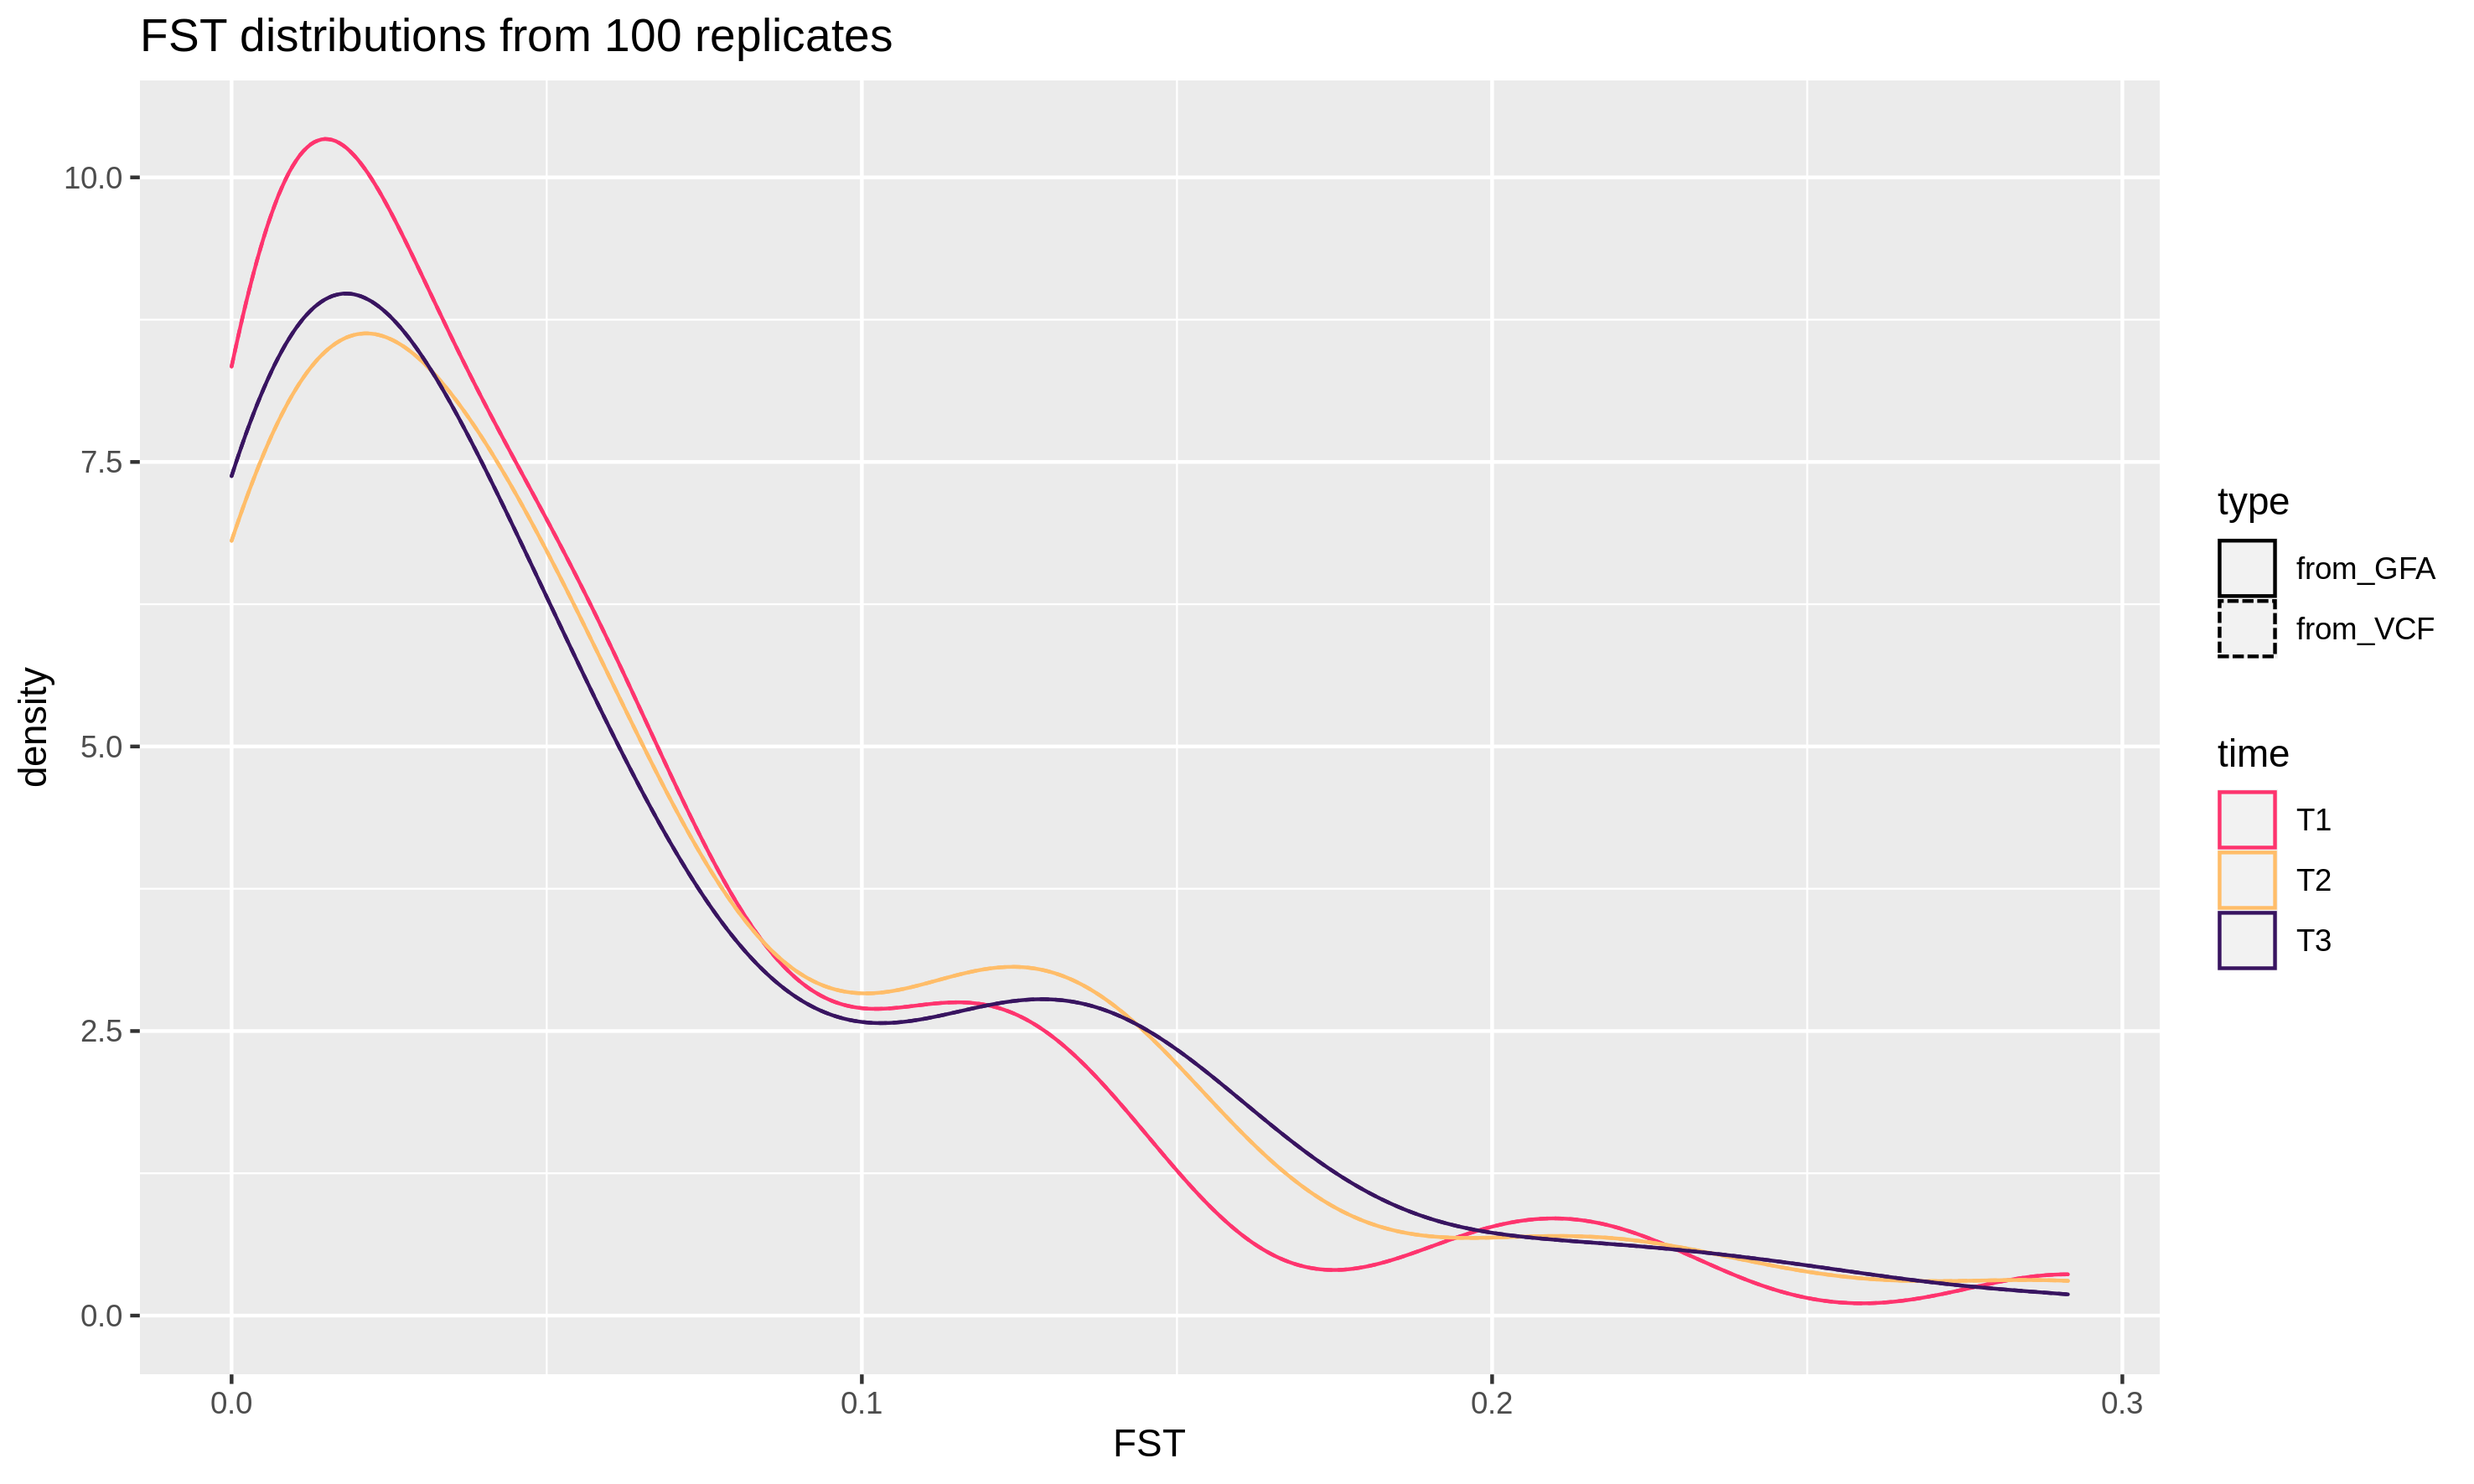
\includegraphics[width=1.00\textwidth]{fig/fst_time (1).png}
\decoRule
\caption{\textbf{Fig:valure of Fst are equal}.}
\label{fig:fsttime.png}
\end{figure}






\section{Study Cases}

I applicate two functions of \vgp to pangenomes of HLA. In particular I calculate \textit{gfa2vcf} and \textit{gfa2allelefreq}.

\subsection{Pangenome HLA}

\begin{figure}[H]
\centering
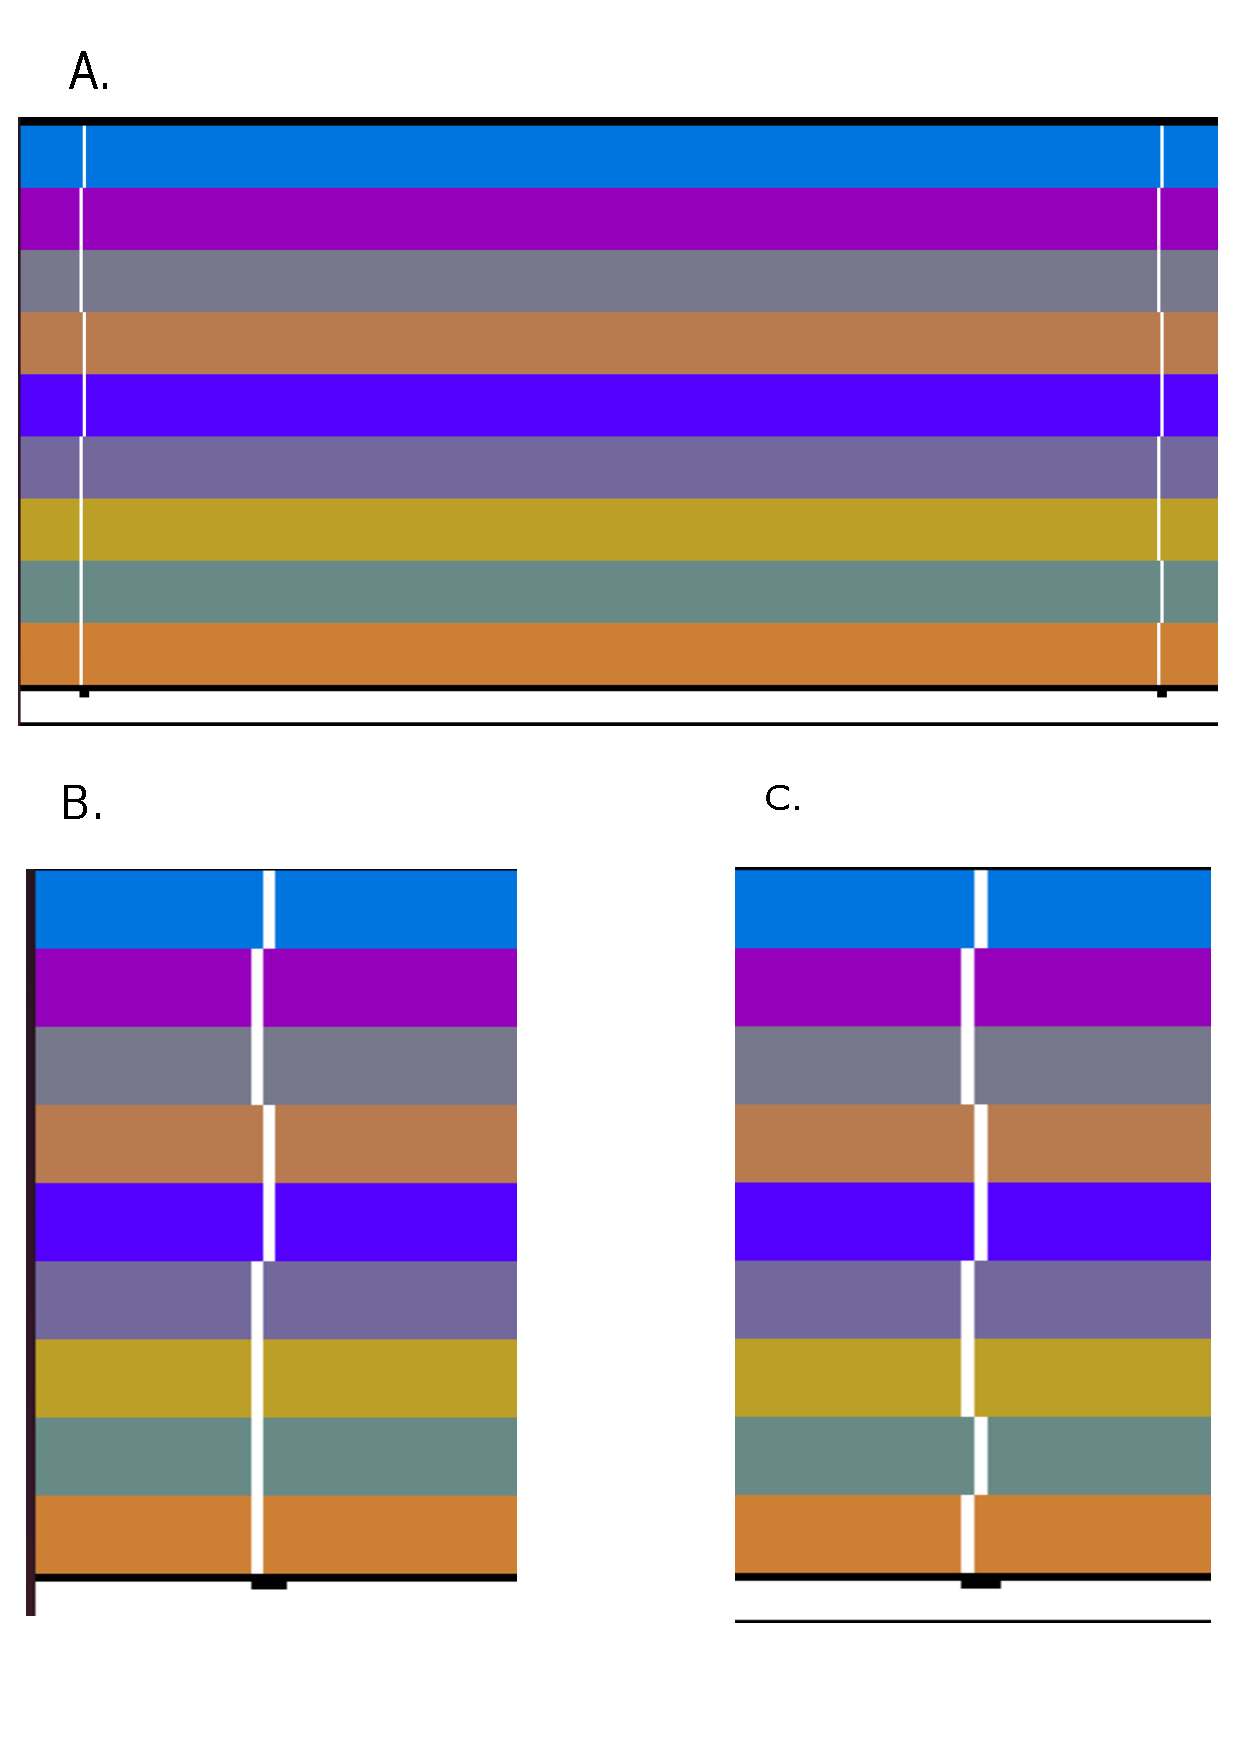
\includegraphics[width=0.50\textwidth]{fig/pangenome.pdf}
\decoRule
\caption{\textit{pangenome}. Is represented a piece of pangenome of HLA, the first row represent Reference and the other rows represent another paths. (\textbf{A}). Zoom for the first column  (\textbf{B}), zoom the second column(\textbf{C})}
\label{fig:pangenome.pdf}
\end{figure}


Pangenomic methods allow us to relate all genomes or sequences in our analysis directly to each other. One of the most polymorphic parts of the genome is the HLA region and for this thing I chose this region.

\subsection{gfa2vcf}

I build pangenome of HLA (see methods) and for the first time I calculate \textit{gfa2vcf}, I convert with odgi GFAformat in an odgiformat. I applicate this function and I obtained VCF.

\begin{verbatim}
odgi build -g E-3133.gfa -o E-3133.og
\end{verbatim}

For validate this result I use vg.
\begin{verbatim}
vg view -Fv E-3133.gfa > E-3133.vg
vg index E-3133.vg -x E-3133.xg
vg deconstruct -p "gi|568815592:30489405-30494204" E-3133.xg
\end{verbatim}

The results are the same.

\subsection{gfa2allelefreq}

The aim is calculate allele frequencies directly on a pangenome. \\

This calculation start with \textit{bubblepop}, after detection of  bubble I calculate allele frequencies, for each variants the number of paths are calculate that support the variant node divided by total number of paths (considered even REF).\\

In this figure ((\ref{fig:pangenome.pdf})A), the first row of the figure represent reference and other rows paths.
Fig: (\ref{fig:pangenome.pdf}A)  for the column in white: first row represent REF, the left node in the REF there isn't in six path, in fact for calculate allele frequencies six paths are divided with 9, the result is 0.66 (\ref{tab:gfa2freqandvcf}first row).


The same for the second column, left node there aren't in 5 paths, and for calculate allele frequencies I divided 5 paths for the total of paths i.e  9, the result is 0.56.


%sequenze nel pangenoma sotto forma di lettere


{\small
\begin{table}
\caption{gfa2freqandvcf}
\label{tab:gfa2freqandvcf}
\centering
\begin{adjustbox}{width=1.00\textwidth}
\begin{tabular}{c c c c c}
\toprule
\tabhead{CHROM} & \tabhead{POS} & \tabhead{REF} & \tabhead{ALT} & \tabhead{FREQ} \\
\midrule
gi|568815592:30489405-30494204 & 551 & 	T & C & 0.67\\
gi|568815592:30489405-30494204 & 883 & G & A & 0.56\\
gi|568815592:30489405-30494204 & 1141 & T & A & 0.11 \\
gi|568815592:30489405-30494204 & 3904 & G & A & 0.67\\
\bottomrule\\
\end{tabular}
\end{adjustbox}
\end{table}
}










% Chapter discussion

\chapter{Conclusions and Future Perspectives-3/6pagine} % Main chapter title

\label{Chapter6} % For referencing the chapter elsewhere, use \ref{Chapter4} 

%----------------------------------------------------------------------------------------

 Discute il significato dei risultati ottenuti dal candidato nell’ambito della problematica e della letteratura scientifica di riferimento, delineando i possibili sviluppi futuri del progetto di ricerca.



Developed  open 
 

% Chapter discussion

\chapter{Materials and Methods}  %(5-10 pagine} % Main chapter title

\label{Chapter7} % For referencing the chapter elsewhere, use \ref{Chapter7} 

%----------------------------------------------------------------------------------------
% Define some commands to keep the formatting separated from the content 


\section{Bubblepop} 
\subsection{Odgi}

I built the \textit{bubblepop} function utilizing the odgi library(\cite{eizenga2020succinct}).

odgi (Optimized Dynamic Graph Implementation) is based on a node centric encoding of the graph that is designed to improve cache coherency when traversing or modifying the graph. This encoding is split between graph topology and paths, which is important for achieving a good balance of run time performance and memory usage on real-world graphs with large path sets. Each node’s sequence and edges are encoded in a byte array using a variable-length integer encoding scheme. Edges are described in terms of a relative offset between the rank of this node in the sorted array of nodes of the graph and the node to which the edge arrives.

The first step is convert the graph in GFA format in a graph in odgi format with:

\begin{verbatim}
odgi build -g graph.gfa -o graph.og
\end{verbatim}

Before executing any of the following commands, initialize the graph object with:

\begin{verbatim}
g=odgi.graph()
\end{verbatim}

Start this function after load GFA, with use two recursive algorithms. 

\subsection{DFS}
Depth first Search is a recursive algorithm for searching all the vertices of a graph or tree data structure.
The DFS algorithm works as follows:

\begin{verbatim}

def dfs(graph, start, visited=None):
    if visited is None:
        visited = set()
    visited.add(start)
    print(start)
    for next in graph[start] - visited:
        dfs(graph, next, visited)
    return visited

\end{verbatim}

\subsection{BFS}
Breadth first Search is a recursive algorithm for searching all the vertices of a tree data structure.
This algorithm works as follows:

\begin{verbatim}
def bfs(graph, root): 
    visited, queue = set(), collections.deque([root])
    visited.add(root)
    while queue: 
        vertex = queue.popleft()
        for neighbour in graph[vertex]: 
            if neighbour not in visited: 
                visited.add(neighbour) 
                queue.append(neighbour) 
\end{verbatim}

I implement this algoritm that is availabe on the git repository of the project. 

%citare: https://www.programiz.com/dsa/graph-bfs 

\subsection{BubblesCalling}

After BFS I continue with a key point of a code, dictionary that identify start and end of bubbles Fig:({\ref{fig:bubblepop.png}}).\\

For define start and end, I calculate distance of node in the three obtained with BFS from root, the chose of root is arbitrary. I use two lists: distance from root and ordinary nodes with the same distance.
Key of a dictionary represent distance and value nodes with the same distance. 

\begin{verbatim}
    
dist_to_num_nodes = dict()   
for node_id, distance in distances_dict.items():
    if distance not in dist_to_num_nodes.keys():   
        dist_to_num_nodes[distance] = 0
    dist_to_num_nodes[distance] += 1

\end{verbatim}

\section{gfa2vcf}

Before run the script GfatoVcf.py, you need to:

1. Convert the GFA format to the ODGI format because this is the format taken as input to the script.
2. With -path specify the path of the odgi library and with -input specify the input file as odgi format

\begin{verbatim}
 python GfatoVcf.py -path /../odgi/lib/ -input /../input.odgi   
\end{verbatim}
    
This code start with the dictionary that there is in \textit{bubblepop}, I continue to identify SNV and INDEL.
\subsection{Extracting Variant and VCF}

\begin{itemize}
\item Chose path as REF: I chose a path (or paths) from the beginning by recording sequences, it is corresponds to REF. Sequence not present in REF, the center of bubble is ALT.


                    
\item Deletion in VCF: If the succ node in the (path that I chose as REF) REF is the current node in the current path, it means that in the current path a node is missing, so there is a DELETION respect to the reference.

\item Insertion in VCF: If the succ node in the current path there is a node in the REF, it means that in the current path there is a node that is missing in the REF, that is an INSERTION.

\item SNV in VCF: Else if sequence is different from the same node in REF and ALT, it is a SNV.

\item POS in VCF: Length of sequence in a node corresponds to POS.
POS, for example (NODE1 ATG)POS is 3 (length of sequence); for (NODE2 AT) POS is 5 because is the sum of the length of the previous node sequence plus the current node length sequence. \end{itemize}


\begin{figure}[H]
\centering
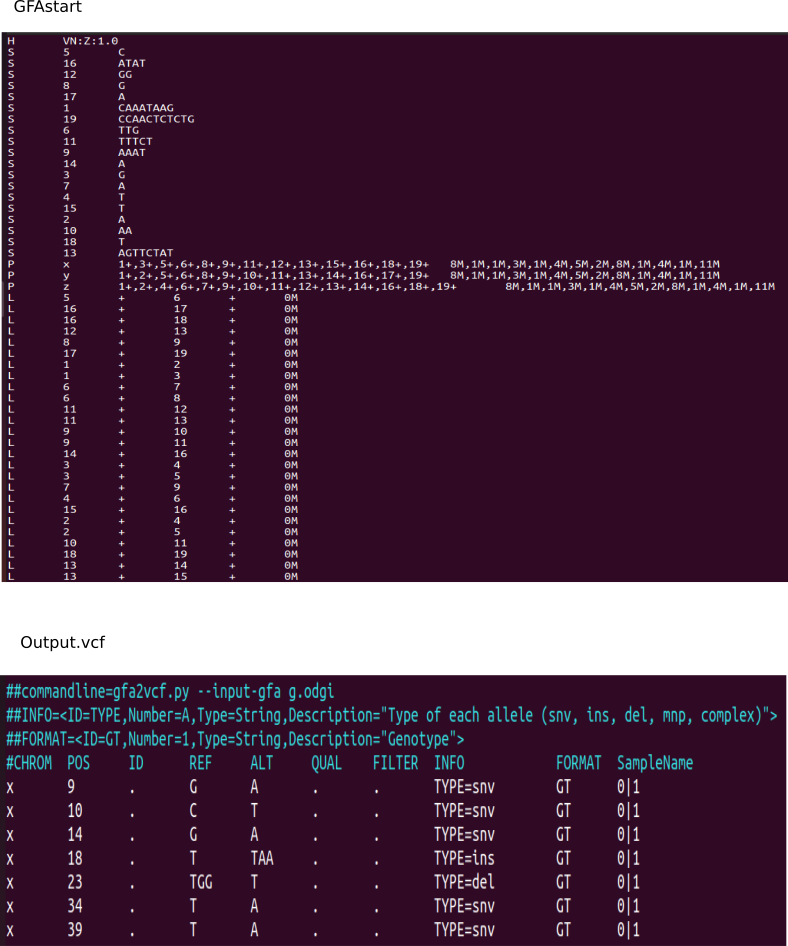
\includegraphics[width=0.70\textwidth]{fig/gfa2vcf.png}
\decoRule
\caption{\textit{GFAstart to VCF} transforms a GFAstart in VCF}
\label{fig:validation.png}
\end{figure}
\subsection{Validation VCF}



I use vg tools for working with genome variation graphs for validate VCF obtained from GFA. 

VCF files generated by \textit{gfa2vcf} is compressed and indexed. Compression optimizes files storage and transfer. Indexing allows fast access to large files. 
\begin{itemize}
\item Compress and indexing
\end{itemize}

Compression was done using Bgzip (\url{https://www.htslib.org/doc/bgzip.html#DESCRIPTION}) that "compresses files into a series of small (less than 64K) 'BGZF' blocks. This allows indexes to be built against the compressed file and used to retrieve portions of the data without having to decompress the entire file"

\begin{verbatim}
~/bin/bgzip output.vcf > output.vcf.gz
\end{verbatim}

Indexing was done using Tabix (\url{https://www.htslib.org/doc/tabix.html}) that "indexes a TAB-delimited genome position file in.tab.bgz and creates an index file". 
The command line takes in input the compressed file from BGZIP and produces an indexed file: 

\begin{verbatim}
~tabix -h output.vcf.gz  
\end{verbatim}

\begin{itemize}
\item  vg construct and view
\end{itemize}
I use indexed file as input of vg construct with reference that I chose. For obtained this output represent in Fig: ( \ref{fig:validation.png} B). I use vgview.

\begin{verbatim}
vg construct -v output.vcf.gz -r reference.fa > VcftoGraph.vg

vg view -dp VcftoGraph.vg | dot -Tpdf -o ValidationGraph.pdf


\end{verbatim}

\section{bcftools and vcftools}

With seqgen2gfa+vcf, I'm starting with Seq-Gen and I obtained GFAformat and VCFformat. 

For calculate allele frequencies on VCF that I obtained from Seq-Gen I use bcftools and vcftools.

\begin{itemize}
    \item Bgzip and Tabix for each replicates

\begin{verbatim}
for f in ./*.vcf; do bgzip "$f"; done   
for f in ./*.vcf.gz; do tabix -h "$f"; done
\end{verbatim}



\item bcftools

Extracting individuals of two populations was done using bcftools (\url{http://samtools.github.io/bcftools/bcftools.html#view})  is a set of utilities that manipulate variant calls in the Variant Call Format (VCF) and its binary counterpart BCF.  I extract individuals with view " subset and filter VCF or BCF files by position and filtering expression".


\begin{verbatim}
parallel bcftools view -S pop_1.txt seqgen_rep{1}.vcf.gz
-o seqgen_rep{1}.pop1.bcf.vcf.gz ::: {1..100} 

parallel bcftools view -S pop_2.txt seqgen_rep{1}.vcf.gz 
-o seqgen_rep{1}.pop2.bcf.vcf ::: {1..100}  
\end{verbatim}

\item vcftools

Calculate allele frequencies from two populations was done using vcftools (\url{http://http://vcftools.sourceforge.net/man_latest.html}), vcftools is a suite of functions for use on genetic variation data in the form of VCF and BCF files. The tools provided will be used mainly to summarize data, run calculations on data, filter out data, and convert data into other useful file formats.

\begin{verbatim}
parallel vcftools --gzvcf seqgen_rep{1}.pop1.bcf.vcf.gz 
--freq --out ms_rep{1}.bcf.pop1.vcf ::: {1..100} 

parallel vcftools  --gzvcf seqgen_rep{1}.pop2.bcf.vcf.gz --freq 
--out ms_rep{1}.bcf.pop2.vcf ::: {1..100}  
\end{verbatim}


%calculate fst, with script fstonvcf

\end{itemize}


\section{Visualization results of Fst from GFA and VCF}

I use R for visualitazion of Fst \ref{fig:fsttime.png}

Import t1,t2,t3 i.e three time of separation of two populations.

\begin{verbatim}

w <- as.data.frame(rbind(t1, t2, t3))
w$time <- c("T1", "T2", "T3")
myd <-w %>% gather(fst, obs, V1:V100)
myd$type<-"from_VCF"

q <- as.data.frame(rbind(t1, t2, t3))
q$time <- c("T1", "T2", "T3")
myd2 <-q %>% gather(fst, obs, V1:V92)

myd2$type<-"from_GFA"

final<-rbind(myd, myd2)

ggplot(final, aes(obs, color=time, linetype=type)) + geom_density() + xlab("FST") + ggtitle("FST distributions from 100 replicates") +scale_color_manual(values=c("#fe346e", "#ffbd69", "#381460"))

 ggsave("fst_time.png", width = 25, height = 15, units = "cm")
 
\end{verbatim}

\section{pangenome HLA}

\begin{itemize}
   

I will use tools supporting the variation graph data model, as described at the pangenome tools (\url{https://pangenome.github.io/}), to build pangenome data from HLA genomes.\\

I start with 9 sequences from chr6 Homo Sapiens, downloads its in formato fasta file. 


\item minimap 
I use (\url{https://lh3.github.io/minimap2/minimap2.html}), is a fast sequence mapping and alignment program that can find overlaps between long noisy reads, or map long reads or their assemblies to a reference genome optionally with detailed alignment. 

I use minimap and I obtained paf format file and bgzip it.

\begin{verbatim}
minimap2 -t 16 -c -X $f $f |gzip > HLA/$b.paf.gz 
\end{verbatim}


\item seqwish and fpa
The alignment to variation graph inducer seqwish \url{https://github.com/ekg/seqwish} renders a set of sequences and alignments into the equivalent variation graph.
Seqwish supports minimap2's PAF format output.
With fpa (filtrare allineamenti sotto 3kb)
    
\begin{verbatim}
seqwish -s HLA/$b.fa.gz -p <(zcat HLA/$b.paf.gz fpa drop -l 2000) -g HLA-gfas/$b.gfa -P
\end{verbatim}
  
\item odgi
With odgi build command constructs a succinct variation graph from a GFA. Currently, only GFA1 is supported.


With odgi sorts a succinct variation graph, sort for have a sort visualization.


With odgi viz I visualize pangenome and save ordinate pangenome. 

\begin{verbatim}
odgi build -g HLA-gfas/$b.gfa -o - | odgi sort -i - -o - -p Ygs -t 16 -P > HLA-gfas/$b.sort.odgi 
odgi viz -i HLA-gfas/$b.sort.odgi -o HLA-gfas/$b.sort.odgi.png -x 4000 -y 500 -R
odgi view -i HLA-gfas/$b.sort.odgi -g > HLA-gfas/$b.sort.gfa
\end{verbatim}

\item VCF and Allelefrequencies

I applicate \textit{gfa2vcf} and I obtained VCF.

\begin{verbatim}
GfatoVcf.py -input E-3133.og -path odgi
\end{verbatim}

For validate this result I use vg.

\begin{verbatim}
vg view -Fv E-3133.gfa > E-3133.vg
vg index E-3133.vg -x E-3133.xg
vg deconstruct -p "gi|568815592:30489405-30494204" E-3133.xg 
\end{verbatim}

I obtained the same result. 

For visualize (\ref{fig:pangenome.pdf}) I use this commands:

\begin{verbatim}
odgi sort -i E-3133.og  -o - | odgi viz -i - -o E-3133.sorted.png -x 15000
\end{verbatim}
\end{itemize}

  


%%%%%%%%%%%%%%%%%%%%%%%%%%%%%%%%%%%%%%%%%%%%%%%%%%%%%%%%%55
% quello sotto VA NEI METODI 
On GFA file I calculate the allele frequencies with \textit{gfa2allelefreq}, the genotype frequencies with \textit{gfa2genofreq}, and the Fst with \textit{gfa2fst}. 

On VCF file I extract individuals from the populations that I considered with bcftools. %non so se mettere questa parte
\begin{verbatim}

bcftools view -S pop_1.txt seqgen.vcf.gz -o seqgen.bcf.vcf.gz #pop1
bcftools view -S pop_2.txt seqgen.vcf.gz -o  seqgen.bcf.vcf  #pop2 
\end{verbatim}

Calculate Allele Frequencies for two populations with vcftools
\begin{verbatim}

vcftools --vcf seqgen.bcf.vcf --freq --out seqgen.bcf.pop1.vcf .frq

vcftools --vcf ms_rep{1}.bcf.vcf --freq --out seqgen.bcf.pop2.vcf.frq 

\end{verbatim}


%\printglossary

\printbibliography[heading=bibintoc]

\begin{acknowledgements}
\addchaptertocentry{\acknowledgementname}
\end{acknowledgements}

\end{document}